\section{Checking whether a given bug is actually real}

Previous sections have described how to generate {\StateMachines}
which represent a given fragment of the program, and how to simplify
them down to remove most of the redundant information.  This section
gives a mechanism for using those {\StateMachines} to check whether
running two fragments of the program in parallel might conceivably
lead to a crash and, if so, under what circumstances it might do so.

The core of the approach is to take a pair of {\StateMachines}, one
representing the read thread and the other representing the write
thread, and convert them into a verification condition using symbolic
execution.  This verification condition is satisfiable precisely when
running the fragments of program represented by the two
{\StateMachines} in parallel might lead to the bug being investigated
reproducing.  Note, though, that this process does not consider the
existing synchronisation present in the program i.e. it is
synchronisation context insensitive, and this can lead to a
significant number of false positives.  See
section~\ref{sect:reproducing_bugs} for one possible way of
eliminating these.

SLI's completeness property is that if every possible \StateMachine
pair which could be generated by the above algorithm is generated and
each one is successfully converted to a verification condition
(i.e. no part of the analysis times out), and none of the verification
conditions are satisfiable, and the dynamic analysis is complete, the
program will not contain any bugs of the class being investigated.

The verification conditions generated here have three main components
which correspond closely to the clauses of the bug definition in
section~\ref{sect:finding_bugs:finding_candidate_bugs:formal_definition}.
These are:

\begin{itemize}
\item
  R atomic -- specifies that the read-side {\StateMachine} must
  predict survival when run atomically.  This translates into a
  precondition on the initial state of the program which is satisfied
  precisely when running the read-side of the purported bug in
  isolation would not crash.
\item
  W atomic -- specifies that when the write-side {\StateMachine} is
  run to completion followed by the read-side {\StateMachine} the
  read-side {\StateMachine} must not predict a crash.  This translates
  into a further precondition which is true for initial states which
  the write-side {\StateMachine} will transform into states which
  satisfy the R atomic precondition.
\item
  Crash possible -- requires that interleaving the two
  {\StateMachines} might cause the read-side {\StateMachine} to
  predict a crash.  This is translated into a predicate over both the
  initial state and the program's happens-before graph which will be
  satisfied for those executions which crash due to the bug which is
  being investigated.
\end{itemize}

\todo{``Initial state'' is arguably a slightly deceptive term here
  because it can include things like control-flow properties of an
  execution of the program.}  The final verification condition is the
conjunction of these three preconditions, and a bug is reported if
that condition is satisfiable.

{\Technique} uses symbolic execution over slightly different
{\StateMachines} to build all of the individual predicates:

\begin{itemize}
\item R atomic is built by symbolically executing the read-side
  {\StateMachine} in isolation and taking the disjunction of the path
  constraints for all paths which reach the \state{Survive} state.
  Note that paths which reach the \state{Unreached} state are treated
  identically to those which reach the \state{Crash} state: these
  paths do not need to be considered by the later phases of analysis,
  by the definition of the \state{Unreached} state, and excluding them
  here makes the later symbolic executions somewhat simpler.
\item W atomic is built by concatenating the two machines and
  symbolically executing the result.  Again, \state{Unreached} states
  are treated identically to \state{Crash} ones.  {\Technique} assumes
  that R atomic holds during the W atomic symbolic execution, which
  can sometimes usefully reduce the set of paths which must be
  considered.
\item Crash possible is produced by symbolically executing the
  cross-product of the two {\StateMachines} and taking the disjunction
  of all paths which reach the \state{Crash} state.  This time, the
  \state{Unreached} state is treated as the \state{Survive} one,
  so as to avoid reporting bugs when the cross-product machine
  reaches a state which is supposed to be ignored.
\end{itemize}

Note that the intermediate {\StateMachines} used here are subject to
the usual simplifications before being symbolically executed, even
though both input {\StateMachines} will have already been simplified
as far as possible.  This can sometimes allow further useful
simplifications and hence reduce the cost of the symbolic execution.
In particular, the simplifiers can assume that no other threads will
interfere with the two threads being executed, which can be very
useful in solving aliasing problems.

The next few sections give some details of the symbolic execution
techniques used and a description of the algorithm used to build the
cross-product {\StateMachine}.

\subsubsection{Symbolically executing machines}

SLI uses a simple symbolic execution engine to evaluate machines and
determine when {\StateMachines} will crash.  The details of this are
fairly standard, and I give only a brief overview
here\editorial{\emph{Should} only give a brief overview; this ended up
  much more detailed than I'd expected.}.  The core data structure
used by the execution engine is a queue of (mostly) symbolic
configurations which the {\StateMachine} might occupy, and the main
operation is to take a state out of this queue, determine what the
\StateMachine might do next, and possibly add some additional
configurations to the queue to explore further.  Each configuration
contains:

\begin{itemize}
\item
  A mapping from {\StateMachine} variables to the (symbolic) values of
  those variables.
\item
  A reference to the {\StateMachine}'s current (non-symbolic) state.
\item
  The order in which those temporaries were assigned to.  As discussed
  in \S~\ref{sect:ssa}, SLI uses a slightly unusual form of single
  static assignment in which $\Phi$ nodes select their input variable
  based on which was assigned to most recently, rather than based on
  the preceding control flow, and this keeping track of that ordering
  allows that semantics to be implemented simply.
\item
  A log of all of the memory stores issued by the \StateMachine so far.
\item
  The current path constraint.  This is simply the conjunction of all
  of the conditions which are known to be true at this point in the
  execution.
\end{itemize}\editorial{Plus some debug crap, but we don't care about that here.}

A symbolic execution will eventually reach one of the {\StateMachine}
terminal states: survive, crash, or unreached.  As discussed above,
the unreached state can be treated as either surviving or crashing,
depending on how the results of the symbolic execution are to be used.
``Impossible'' paths, such as those where the {\StateMachine}
dereferences a bad pointer, are treated as if they reached the
unreached state\footnote{Note the program dereferencing a bad pointer
  does not imply that the {\StateMachine} does as well.  In
  particular, if the {\StateMachine} was generated to investigate a
  bad pointer dereference at memory accessing-instruction $I$ then $I$
  will be translated into a test of a $BadPtr$ expression, rather than
  a memory access, and so will never cause the {\StateMachine} to
  dereference a bad pointer.}.

Implementing the various types of \StateMachine operation is
straightforward:

\begin{itemize}
\item Conditional branches.  The condition in the branch is compared
  to the path constraint to determine whether the branch is completely
  determined by the path constraint.  If it is, execution simply moves
  to the appropriate successor state.  Otherwise, two new successor
  configurations are added to the queue, one for the true branch of
  the conditional and the other for the false branch, and the path
  constraints updated as appropriate.
\item \state{Copy} $var = expr$, which evaluates $expr$ ands store it
  in the {\StateMachine}-level variable $var$.  The expression is
  simplified as far as possible using the information in the path
  constraint and stored in the appropriate place in the variable
  table.  The variable is then moved up in the variable assignment
  order table.
\item \state{Store} $value \rightarrow \ast(addr)$, which evaluates
  $addr$ and $value$ and stores the value of $value$ to the memory
  location $addr$.  The symbolic executor simplifies $addr$ and
  $value$ using the path constraint and then adds a new entry to the
  end of the memory store log.

  Depending on the mode of operation, the engine might also test
  whether $addr$ is a bad pointer and, if it is, branch to the
  unreached state, much as it would if the {\StateMachine} had
  asserted $\not{}BadPtr(addr)$.  This extra assertion can then
  sometimes be used to simplify $BadPtr$ expressions which occur later
  in the {\StateMachine}'s execution.  This is often useful if the bug
  to be investigated is itself a bad pointer dereference but tends to
  be less so if the bug is an assertion failure, and so the engine
  only does this in the former case.

\item \state{Load} $\ast(addr) \rightarrow var$, which evaluates
  $addr$ to the address of a memory location and then copies the
  current contents of that location to the {\StateMachine} variable
  $var$.  As usual, symbolic execution starts by simplifying $addr$
  using the path constraint.  The resulting address is then compared
  to every location in the store log to determine which stores might
  possibly satisfy the load and a successor configuration created for
  each.  Each of these successor configurations will have $var$ set to
  an appropriate value and the path constraint extended with enough
  additional clauses to ensure that the \state{Load} is satisfied by
  the desired \state{Store}.  There may also be an additional
  successor configuration for the case where the \state{Load} does not
  match any \state{Store}s and instead returns the initial contents of
  memory, with appropriate values for $var$ and appropriate
  modifications to the path constraint.

  As for \state{Store} operations, \state{Load}s may sometimes also
  introduce a constraint that the dereferenced pointer is valid, if
  the symbolic execution engine is being used in a mode where that is
  likely to be helpful.

\item \state{$\Phi$} $\{var_1,var_2,\ldots{},var_n\} \rightarrow var$
  selects whichever of the $var_i$ inputs has been most recently
  assigned to and copies its value to $var$.  This is simple to
  implement given that each configuration includes a log of the order
  in which variables are assigned to and produces a single successor
  configuration.

\item
  Every other operation is a no-op in the interpreter and simply moves
  to the next state.  In particular, the execution engine ignores
  operations such as \state{StackLayout} and \state{PointsTo} which
  simply provide additional hints to the various \StateMachine
  simplification phases.  One might expect that these would be useful
  for determining which \state{Store} should be used to satisfy a
  given \state{Load} operation, but in almost all cases where these
  hints provide useful information the {\StateMachine} simplification
  passes will have already used it to simplify the {\StateMachine},
  and so there is little to be gained from repeating the analysis
  here.

  The \state{StartAtomic} and \state{EndAtomic} states are also
  treated as no-ops in the symbolic execution engine.  This is because
  the engine only ever processes a single {\StateMachine} at a time,
  and so the entire {\StateMachine} is already implicitly atomic.

  \todo{Actually, the effects get stripped out before we start, rather
    than ignored here, but it ends up being equivalent.}
\end{itemize}

\todo{The path constraint is initialised to whatever assumptions we're
  allowed to make when the symbolic execution starts, so R atomic when
  we're trying to derive W atomic.}

\todo{Surprise: you basically never re-visit an old configuration in
  this model.  Not sure why that is, and it's almost certainly not a
  good thing.}

\subsection{Building cross-product {\StateMachines}}
\label{sect:using:build_cross_product}

The symbolic execution engine is only capable of exploring one
{\StateMachine} at a time, and so if cross-thread behaviours are to be
investigated then the single-threaded {\StateMachines} must be
combined into a single multi-threaded one.  This is trivial for the
{\StateMachine} used in deriving W atomic (the two {\StateMachines}
are concatenated together by replacing the terminal state of the
write-side {\StateMachine} with the a copy of the read-side
{\StateMachine}), but the one used to derive the crash-possible
constraint is somewhat more involved.  The obvious approach here would
be to a cross-product of the two {\StateMachines}, but this would be
both inefficient, due to the presence of partial order
redundancies\needCite{}, and incorrect, due to the presence of atomic
blocks within the {\StateMachines}.  {\Technique}'s approach is a
refinement of the cross-product algorithm which avoids this
incorrectness while also mitigating the inefficiency.  It also avoids
running either {\StateMachine} to completion before the other starts,
since the results obtained from executing such a path would be
immediately discarded by the R atomic and W atomic preconditions.

\todo{I want to explain this in terms of supercompilation of an
  abstract interpreter, but it's not quite coming together.}

The algorithm used is actually rather simple.  The core idea is to
identify each state of the output {\StateMachine} with a particular
configuration of the two input {\StateMachines}, where the
configuration contains all of the necessary information about the
concurrent interleaving of the two {\StateMachines} and nothing else.
More concretely, a configuration consists of five fields:

\begin{itemize}
\item The {\StateMachine} state which each machine is to execute next;
\item A field saying which, if any, of the input {\StateMachines} are
  currently in atomic blocks;
\item A flag indicating whether the read-side {\StateMachine} has
  issued any memory accesses yet; and
\item A flag indicating whether the write-side {\StateMachine} has
  issued any stores.
\end{itemize}

The output machine starts in a configuration with both input
{\StateMachines} in their initial state, neither in an atomic block,
and neither having issued any memory accesses.  The algorithm then
exhaustively explores every configuration reachable from this one,
building the output {\StateMachine} as it goes.

As an example, consider the {\StateMachines} shown in
figure~\ref{fig:cross_product_input}.  $y$ here is supposed to
indicate some value which is local to the write-side {\StateMachine}
and $x$ some global variable in memory.  These produce the
cross-product {\StateMachine} shown in
figure~\ref{fig:cross_product_output}.  I highlight a couple of the more important
features of this diagram:

\begin{itemize}
\item The {\StateMachine} starts in the configuration (A, E,
  $\varnothing$, false, false), indicating that the read-side
  {\StateMachine} is in state A, write-side one is in state $E$,
  neither one is in an atomic section, and neither has issued any
  memory accesses.  The write-side machine is about to execute a
  thread-local operation and so the cross-product algorithm allows it
  to advance independently.  In this case, that operation is an
  \state{If} state, so the write-side state has two successors, and so
  the configuration has two successor configurations.
\item One of the successors of this initial state is (A, I,
  $\varnothing$, false, false).  Here, the write-side {\StateMachine}
  has reached a terminal state I before the read-side {\StateMachine}
  issued any memory accesses, as indicated by the first false, and so
  the output state is \state{Unreached} and no further exploration is
  necessary.  Likewise all of the other ways in which one
  {\StateMachine} could complete before the other starts have been
  converted to \state{Unreached} and will be removed by the
  simplifier.
\item In the other success of the initial state, (A, F, $\varnothing$,
  false, false), both {\StateMachines} have reached a memory accessing
  state.  The cross-product algorithm now uses a happens-before test
  to incorporate both possible orderings of these accesses into the
  output {\StateMachine}.  In this way all of the relevant memory
  ordering behaviour of the two input {\StateMachines} is incorporated
  into the output {\StateMachine}.
\item The output {\StateMachine} might no longer be in static single
  assignment form.  This can sometimes reduce the effectiveness of
  {\StateMachine} simplifications on the output {\StateMachine}.

  \todo{This kind of sucks.  I need to think of something clever to
    say here.}

\item In this case, simplification will be effective and will reduce
  the {\StateMachine} to that shown in
  figure~\ref{fig:cross_product_output_opt}; symbolic execution is
  barely necessary to determine the crash constraint.  More complex
  {\StateMachines} will not simplify nearly so well. \todo{Not sure I
    really needed to say that.}
\end{itemize}

\begin{figure}
  \begin{subfloat}
    \begin{tikzpicture}
      \node[stateSideEffect,initial] (lA) {lA: \state{Load} $x \rightarrow tmp$ };
      \node[stateIf,below = of lA] (lB) {lB: \state{If} $tmp = 0$ };
      \node[stateSideEffect,below = of lB] (lC) {lC: \state{Load} $x \rightarrow tmp'$ };
      \node[stateIf,below = of lC] (lD) {lD: \state{If} $BadPtr(tmp')$ };
      \node[stateTerminal,below = of lD] (lH) {lH: \state{Crash} };
      \node[stateTerminal,right = of lC] (lG) {lG: \state{Survive} };
      \draw[->] (lA) -- (lB);
      \draw[->] (lB) to node {true} (lG);
      \draw[->] (lB) to node {false} (lC);
      \draw[->] (lC) -- (lD);
      \draw[->] (lD) to node {true} (lH);
      \draw[->] (lD) to node {false} (lG);
    \end{tikzpicture}
    \caption{Read-side}
  \end{subfloat}
  \begin{subfloat}
    \begin{tikzpicture}
      \node[stateIf,initial] (lE) {lE: \state{If} $y \not= 0$};
      \node[stateSideEffect,below right = of lE] (lF) {lF: \state{Store} $0 \rightarrow x$};
      \node[stateTerminal,below left = of lF] (lI) {lI: \state{Survive} };
      \draw[->] (lE) to node {true} (lI);
      \draw[->] (lE) to node {false} (lF);
      \draw[->] (lF) -- (lI);
    \end{tikzpicture}
    \caption{Write-side}
  \end{subfloat}
  \caption{Some {\StateMachines}.  $x$ is a global memory location.}
  \label{fig:cross_product_input}
\end{figure}

\begin{figure}
  \begin{tikzpicture}[align=center]
    \node[stateIf, initial] (A) {(A, E, $\varnothing$, false, false)\\\state{If} $y \not= 0$ };
    \node[stateTerminal, right = of A] (B) {(A, I, $\varnothing$, false, false)\\\state{Unreached} };
    \node[stateIf, below = of A] (C) {(A, F, $\varnothing$, false, false)\\\state{If} $A \happensBefore F$ };
    \node[stateSideEffect, below = of C] (D) {\state{Load} $x \rightarrow tmp$};
    \node[stateSideEffect, right = of C] (E) {\state{Store} $0 \rightarrow x$};
    \node[stateIf, below = of D] (F) {(B, E, $\varnothing$, true, false)\\\state{If} $tmp = 0$ };
    \node[stateTerminal, below = of E] (G) {(A, I, $\varnothing$, false, true)\\\state{Unreached} };
    \node[stateTerminal, right = of F] (H) {(G, E, $\varnothing$, true, false)\\\state{Unreached} };
    \node[stateIf, below = of F] (I) {(C, E, $\varnothing$, true, false)\\\state{If} $C \happensBefore F$ };
    \node[stateSideEffect, below = of I] (J) {\state{Load} $x \rightarrow tmp'$};
    \node[stateSideEffect, right = of I] (K) {\state{Store} $0 \rightarrow x$};
    \node[stateIf, below = of J] (L) {(D, E, $\varnothing$, true, false)\\\state{If} $BadPtr(tmp')$ };
    \node[stateSideEffect, right = of K] (M) {(C, I, $\varnothing$, true, true)\\\state{Load} $x \rightarrow tmp'$ };
    \node[stateTerminal, below = of L] (N) {(H, E, $\varnothing$, true, false)\\\state{Unreached} };
    \node[stateTerminal, below right = of L] (O) {(G, E, $\varnothing$, true, false)\\\state{Unreached} };
    \node[stateIf, below = of M] (P) {(D, I, $\varnothing$, true, true)\\\state{If} $BadPtr(tmp')$ };
    \node[stateTerminal, left = of P] (Q) {(G, I, $\varnothing$, true, true)\\\state{Survive} };
    \node[stateTerminal, below = of P] (R) {(G, I, $\varnothing$, true, true)\\\state{Crash} };
    \draw[->] (A) to node {true} (B);
    \draw[->] (A) to node {false} (C);
    \draw[->] (C) to node {true} (D);
    \draw[->] (C) to node {false} (E);
    \draw[->] (D) -- (F);
    \draw[->] (E) -- (G);
    \draw[->] (F) to node {true} (H);
    \draw[->] (F) to node {false} (I);
    \draw[->] (I) to node {true} (J);
    \draw[->] (I) to node {false} (K);
    \draw[->] (J) -- (L);
    \draw[->] (K) -- (M);
    \draw[->] (L) to node {true} (N);
    \draw[->] (L) to node {false} (O);
    \draw[->] (M) -- (P);
    \draw[->] (P) to node {true} (Q);
    \draw[->] (P) to node {false} (R);
  \end{tikzpicture}
  \caption{Cross product of the {\StateMachines} shown in
    figure~\ref{fig:cross_product_input}. \todo{redo layout} }
  \label{fig:cross_product_output}
\end{figure}

\begin{figure}
  \begin{tikzpicture}[align=center]
    \node[stateSideEffect, initial] (A) {\state{Assert} $y = 0 \wedge A \happensBefore F \wedge LD(x) \not= 0 \wedge F \happensBefore C$ };
    \node[stateTerminal, below = of A] (B) {\state{Crash} };
    \draw[->] (A) -- (B);
  \end{tikzpicture}
  \caption{Result of simplifying {\StateMachine} shown in figure~\ref{fig:cross_product_output}.}
  \label{fig:cross_product_output_opt}
\end{figure}

The algorithm used in $\implementation$ has a number of other features
not illustrated here:

\begin{itemize}
\item
  Atomic blocks are correctly maintained.  Issuing a
  \state{StartAtomic} side-effect causes the third field of the label
  tuple to be set to the issuing {\StateMachine} and from that point
  only that {\StateMachine} will be allowed to advance until it
  reaches an \state{EndAtomic} side-effect.  

\item
  It is not always necessary to consider both orderings for every
  memory access.  In particular, if the access in one machine cannot
  possibly alias with \emph{any} future access in the other then it is
  safe to dispense with the $\happensBefore$ condition and directly
  issue that access.

  \todo{Shrink this}

  Note that it is \emph{not} safe to simply test the two next accesses
  against each other and skip the $\happensBefore$ test if those two
  accesses happen not to conflict.  TO understand why, consider this
  diagram:

  \begin{tikzpicture}
    \node[draw] (L1) {L1};
    \node[draw, below = of L1] (L2) {L2};
    \node[draw, right = of L1] (S1) {S1};
    \node[draw, below = of S1] (S2) {S2};
    \node[draw, below = of S2] (S3) {S3};
    \draw[->] (L1) -- (L2);
    \draw[->] (S1) -- (S2);
    \draw[->] (S2) -- (S3);
    \draw[<->, dashed] (L1) -- (S2);
    \draw[<->, dashed] (L1) -- (S3);
    \draw[<->, dashed] (L2) -- (S2);
  \end{tikzpicture}

  This is supposed to indicate that the read-side {\StateMachine} has
  two operations, L1 and L2, and the store machine has three, S1
  through S3, and that L1 could alias with S1 or S3 while L2 can only
  alias with S2.  This graph cannot be correctly handled if only
  directly-racing accesses are considered for permutation.  The
  algorithm will start in the configuration (L1, S1, $\varnothing$,
  false, false), and determine that L1 can race with S1 so introduce
  an $\happensBefore$ test to distinguish the two cases.  Consider the
  case where L1 is issued before S1 first.  The algorithm will now
  have to encode a {\StateMachine} for the configuration (L2, S1,
  $\varnothing$, true, false).  L2 does not directly conflict with
  S1, so if only direct races were considered then it would be able to
  issue L2 and S1 in either order.  If it issues L2 first then that
  will lead to the read-side {\StateMachine} completing before the
  write-side one has started, and so all orderings where L1 comes
  before S1 will be ignored.

  Now consider the case where S1 is issued before L1.  The next
  configuration to be considered is then (L1, S2, $\varnothing$,
  false, true), and L1 does not directly interfere with S2, so the
  algorithm can immediately issue S2 and move on to (L1, S3,
  $\varnothing$, false, true).  Now the only option is to issue L1, as
  otherwise the store machine will complete before the load machine
  starts, moving to (L2, S3, $\varnothing$, false, true).  Finally, L2
  does not directly interfere with S3, and so only one ordering of the
  two accesses need be considered; assume the algorithm picks L2
  first.  Now the only access considered by the cross-product
  {\StateMachine} is S1, S2, L1, L2, S3, which clearly does not
  adequately cover the potential interleavings of these two
  {\StateMachines}.

  \todo{Need to mention the magic words ``partial order reduction'' in
    here somewhere.}

\item
  Of course, it is not always entirely clear when two accesses might
  overlap, as the addresses accessed can be completely arbitrary
  expressions.  In that case, the algorithm adds an additional
  assertion to one of the successor states requiring that the accesses
  alias. \todo{Explain why only one.}
\end{itemize}

\subsection{Path explosion}

One common problem in symbolic execution systems is path explosion:
the number of paths through a program rises exponentially in the size
of the program, and this can prevent na\"ive symbolic execution
systems from being applied to realistically large programs.  In the
case of \technique, there are two main causes of path explosion:

\begin{itemize}
\item
  Aliasing.  If the various simplification passes and the dynamic
  analysis cannot determine how memory accessing instructions alias
  then the symbolic execution engine must consider every possible
  aliasing pattern, of which there are $O(n^m)$, where $n$ is number
  of \state{Load} operations and $m$ the number of \state{Store} ones.
  This grows rather quickly in the number of unsolvable aliasing
  problems, especially when the number of \state{Store}s in the
  {\StateMachine} rises.  This represents one of the major limitations
  to \technique's scalability.
\item
  Thread interleaving.  The cross-product {\StateMachine} will have
  $O(nm)$ states, where $n$ is number of states in the read-side
  {\StateMachine} and $m$ the number in the write-side one.  The
  number of paths through the combined {\StateMachine} then grows as
  $O(2^(nm))$, which again grows rather quickly.
\end{itemize}

The result is that, in the common case where the read-side
{\StateMachine} consists mostly of \state{Load} operations and
write-side one mostly of \state{Store} ones, the symbolic execution
engine might have to consider up to $O((2n)^m)$ distinct paths when
evaluating the cross-product {\StateMachine}.  This is obviously
completely infeasible for even moderate values of $n$ and $m$.  For
good performance, {\technique} is completely reliant on the various
simplification and analysis techniques to reduce $n$ and $m$ to
something manageable.  Fortunately, as discussed in the evaluation,
they are able to do so in a useful set of cases.

\subsection{Use of the induction rule}

When analysing a potential crash at instruction $i$, it is sometimes
possible to show that the existence of a bug at $i$ would imply the
existence of a bug at an earlier instruction $i'$.  This allows
{\technique} to use a form of induction to eliminate some potential
bad pointer dereference-type bugs, or at the very lest to reduce the
number of very similar bugs reported.  The idea here is to take the
read-side {\StateMachine} from a candidate bug and truncate it,
cutting it off at some memory-accessing state, in such a way that the
truncated {\StateMachine} will report a crash if the original
{\StateMachine} would have dereferenced a bad pointer at that memory
access.  A new verification condition is then generated using that
truncated {\StateMachine} as the read-side {\StateMachine} and the
original write-side {\StateMachine} as the write-side.  A bug only
needs to be reported for the original pair of {\StateMachines} if
there is some initial state which satisfies the original verification
condition but does not satisfy the truncated one.

Of course, like most forms of induction, this requires a base case in
order to be sound.  The main bug-finding analysis therefore records
every time it had to use the induction rule to eliminate a bug,
including which instruction the eliminated bug was at and which
instruction was assumed to be bug-free in order to eliminate it.  Once
the main analysis is complete this log is checked for cycles.  If it
is cycle free then the induction rule is sound.  I have not, so far,
found any programs for which the graph contains a cycle, but if a
cycle were to be found then it could sensibly be handled by selecting
a single bug from the cycle and reporting that, ignoring all others.

This rule relies on the monotonicity property of the definition of
crashes, as discussed in \S~\ref{sect:monotonicity}.  As such, it is
not sound in the presence of mandatory concurrency, and might lead to
bugs which do not require mandatory concurrency being neglected simply
because they happen to be ``near to'' a bug which does.  As argued
previously, mandatory concurrency should be rare in most programs, and
so I do not expect this to be a problem in practice.  \todo{Might want
  a bit more there?}

\todo{Forward ref eval to say how useful this is.}

\subsection{Completeness}
\todo{I've kind of already covered this, but it might be worth pulling
  all of the completeness discussion together into one place.}

\section{The satisfiability checker}
This doesn't really belong here.  I should figure out where to put it.
I should also figure out whether I'd be better off using someone
else's checker.  The current one is pretty damn stupid; it tries a
couple of normal forms and then if they don't do anything useful does
an implicit analytic tableaux-type thing.

\section{Reproducing bugs}
\label{sect:reproducing_bugs}

\todo{Having written this up, I'm not convinced the idea of message
  payloads is all that useful for describing how cross-thread
  constraints are evaluated.  Nevermind.}

\todo{Should make it explicit that the CFGs we're working with here
  are the unrolled CFGs used when building {\StateMachines}, rather
  than the program's raw CFGs.}

Given a pair of {\StateMachines} and a verification condition it is
also possible to build a ``crash enforcer'' which will insert delays
into the program's execution in a way which will make the bug more
likely to reproduce.  This can then be used to determine which of the
many bugs reported by the prior analysis are actually reproducible,
and hence to appropriately target efforts in fixing them.  In effect,
the {\StateMachine} pair is turned into a custom dynamic analysis
which targets just the bug of interest.

I now illustrate the basic approach with a simple example before
giving details of the algorithms used.  Suppose that the bug to be
exhibited involves two threads:

\begin{verbatim}
int *global_ptr[];
void thread1(int idx1) {
    if (global_ptr[idx1])
        *global_ptr[idx1] = 7;
} 
void thread2(int idx2) {
    global_ptr[idx2] = NULL;
}
\end{verbatim}

Suppose further that these functions compile to this machine code:

\begin{verbatim}
thread1:

l1:   ADD global_ptr + idx1 -> reg1
l2:   LOAD *reg1 -> reg2
l3:   CMP 0, reg2
l4:   jmp_if_eq l7
l5:   LOAD *reg1 -> reg3
l6:   STORE 7 -> *reg3
l7:

thread2:

l8:   ADD global_ptr + idx2 -> reg4
l9:   STORE 0 -> *reg4
\end{verbatim}

There is a risk here that \verb|thread1| might crash if \verb|l9| is
interleaved between \verb|l2| and \verb|l5| and \verb|idx1 == idx2|.
The previous analysis phase will produce \StateMachines something like
these:

\begin{tikzpicture}
  \node[stateSideEffect,initial] (l2) {l2: Load $global\_ptr + idx1$ to $tmp1$};
  \node[stateIf,below = of l2] (l4) {l4: If $tmp1 == 0$?};
  \node[stateSideEffect, below = of l4] (l5) {l5: Load $global\_ptr + idx1$ to $tmp2$};
  \node[stateIf,below = of l5] (l6) {If $BadPtr(tmp2)$?};
  \node[stateTerminal,below right = of l6] (crash) {Crash};
  \node[stateTerminal,below left = of l6] (survive) {Survive};
  \draw[->] (l2) -- (l4);
  \draw[->] (l4) -- node {false} (l5);
  \draw[->] (l5) -- (l6);
  \draw[->] (l4.west) to [bend right=80] node {true} (survive);
  \draw[->] (l6.east) to [bend left=70] node {true} (crash);
  \draw[->] (l6.west) to [bend right=75] node {false} (survive);
  \begin{pgfonlayer}{bg}
    \node(box99) [fill=black!10,fit=(l2) (l4) (l5) (l6) (survive) (crash)] {};
  \end{pgfonlayer}

  \begin{scope} [xshift=8cm,yshift=-3cm]
    \node[stateSideEffect,initial] (l9) {l9: Store $0$ to $global\_ptr + idx2$};
    \node[stateTerminal,below=of l9] (end) {Finish};
    \draw[->] (l9) -- (end);
    \begin{pgfonlayer} {bg}
      \node [fill=black!10,fit=(l9) (end)] {};
    \end{pgfonlayer}
  \end{scope}
\end{tikzpicture}

With a verification condition that $idx1 == idx2 \wedge l2
\happensBefore l9 \wedge l8 \happensBefore l5$.  We can therefore
augment the \StateMachines with happens before edges as shown:

\begin{tikzpicture}
  \node[stateSideEffect,initial] (l2) {l2: Load $global\_ptr + idx1$ to $tmp1$};
  \node[stateIf,below = of l2] (l4) {l4: If $tmp1 == 0$?};
  \node[stateSideEffect, below = of l4] (l5) {l5: Load $global\_ptr + idx1$ to $tmp2$};
  \node[stateIf,below = of l5] (l6) {If $BadPtr(tmp2)$?};
  \node[stateTerminal,below right = of l6] (crash) {Crash};
  \node[stateTerminal,below left = of l6] (survive) {Survive};
  \draw[->] (l2) -- (l4);
  \draw[->] (l4) -- node {false} (l5);
  \draw[->] (l5) -- (l6);
  \draw[->] (l4.west) to [bend right=80] node {true} (survive);
  \draw[->] (l6.east) to [bend left=70] node {true} (crash);
  \draw[->] (l6.west) to [bend right=75] node {false} (survive);
  \begin{pgfonlayer}{bg}
    \node(box99) [fill=black!10,fit=(l2) (l4) (l5) (l6) (survive) (crash)] {};
  \end{pgfonlayer}

  \begin{scope} [xshift=8cm,yshift=-3cm]
    \node[stateSideEffect,initial] (l9) {l9: Store $0$ to $global\_ptr + idx2$};
    \node[stateTerminal,below=of l9] (end) {Finish};
    \draw[->] (l9) -- (end);
    \begin{pgfonlayer} {bg}
      \node [fill=black!10,fit=(l9) (end)] {};
    \end{pgfonlayer}
  \end{scope}

  \draw[->,happensBeforeEdge] (l2.south) -- (l9.north);
  \draw[->,happensBeforeEdge] (l9.south) -- (l5.north);
\end{tikzpicture}

The task is then to modify the program so as to make it more likely
that this happen-before graph will be satisfied when the program runs
while leaving its behaviour otherwise unchanged.  This can be
accomplished by inserting small delays into the program's execution.
In this case, simply inserting a delay before \verb|l5| would probably
be sufficient, as that would enlarge the critical section and hence
make it more likely that the critical store will intervene.

\begin{figure}
  \begin{tikzpicture}
    \node[draw] (A) {A};
    \node[draw, below right = of A] (X) {X};
    \node[draw, below left = of X] (B) {B};
    \node[draw, below right = of B] (Y) {Y};
    \node[draw, below left = of Y] (C) {C};
    \draw[->] (A) -- (B);
    \draw[->] (B) -- (C);
    \draw[->] (X) -- (Y);
    \draw[->,happensBeforeEdge] (A) -- (X);
    \draw[->,happensBeforeEdge] (X) -- (B);
    \draw[->,happensBeforeEdge] (B) -- (Y);
    \draw[->,happensBeforeEdge] (Y) -- (C);
  \end{tikzpicture}
  \caption{A happens-before graph which cannot be reproduced by
    inserting a single delay.}
  \label{fig:enforce_crash:complex_hb}
\end{figure}

More complex happens-before graphs can make it more complex to
determine where delays should be inserted.  Consider, for instance,
the happens-before graph shown in
figure~\ref{fig:enforce_crash:complex_hb}.  This is intended to show
two threads, one which executes instructions A, B and C in order and
the other which executes X and then Y, where the behaviour of interest
only happens with the interleaving A, X, B, Y, C.  There is no simple
critical section structure here, making it less obvious where delays
need to be inserted.  Even once it has been determined where to insert
the delays, deciding their magnitude remains non-trivial: the delay
between X and Y for instance, must be large enough to be confident
that B happens before Y if A happens before X, but not so large that C
is also likely to happen before Y.  Simply picking the largest delay
which avoids unacceptable performance overheads risks masking such
bugs.  Solving such constraints requires a far more detailed model of
the program's structure and the time taken by various instructions,
and such models are both difficult to derive and fragile once they are
available.

SLI solves this problem using a message-passing system.  The core idea
is to model a happens-before ordering X before Y as a message which is
sent by X, after it completes, and collected by Y, before it starts.
These messages are synchronous: the sender will wait for the receiver,
and the receiver will wait for the sender, in both cases with a short
timeout.  In the first example, there will be two messages, one sent
from \verb|l2| to \verb|l9| and the other sent from \verb|l9| to
\verb|l5|.  Delays will be inserted immediately before \verb|l9| and
\verb|l5|, and also immediately after \verb|l2| and \verb|l9|.  These
delays have slightly different functions:

\begin{itemize}
\item
  The delay after \verb|l2| makes the read-side of the critical
  section wait for a matching write-side.  In effect, this delay
  enlarges the read-side critical section in the hope that a
  write-side operation will come along which can be dropped into it.
  This is useful for bugs where the write-side occurs much more
  frequently than the read-side.
\item
  The delay before \verb|l9| makes the write-side wait for a matching
  read-side.  The intuition here is that the enforcer will maintain a
  ``pool'' or write-side operations, which can then be deployed as
  soon as a read-side operation turns up.  This is useful for bugs
  where the read-side occurs much more frequently than the write-side.
\item
  The delays after \verb|l9| and before \verb|l5| help the read- and
  write-sides of the critical section to proceed with the desired
  interleaving.  By this point, the two threads have rendezvoused and
  been bound together, and so there is no need to wait for a matching
  operation to arrive, and the delay is necessary only to wait for the
  paired thread to reach the appropriate place in its control-flow
  graph (or to exit the simulation, causing the message operation to
  fail).  The timeout is in this case necessary only to prevent
  deadlocks: it is possible that the program contains some
  synchronisation structure of which SLI is unaware, so that one
  thread might be waiting for the other, and introducing an additional
  unbounded wait would be unsafe.

  \todo{The difference between bound and unbound message operations is
    important; it deserves more discussion than this.}
\end{itemize}

Setting the sizes of these delays, especially those after \verb|l2|
and \verb|l9|, involves a delicate trade-off between performance and
the likelihood of uncovering bugs.  In general, SLI will choose one of
\verb|l2| or \verb|l9| as a delay-able instruction, according to their
relative frequency, and use a large timeout for the delay-able
instruction and a very small one for the non-delay-able one.  This is
discussed further in section\needCite{}.

Encoding the second example as a message-passing system requires more
message operations but does not introduce any additional conceptual
complexity.

This basic message passing scheme is sufficient to ensure that the
instructions of the program obey the happens-before graph.  That is
sufficient to trigger the desired behaviour in some cases but not all.
In particular, it can be insufficient if there is some additional
non-trivial side-condition required before the bug reproduces, beyond
simply requiring a particular happens-before graph.  Suppose, for
instance, that the read- and write-side {\StateMachines} are
operations on some dynamic structure and that there are many instances
of the structure in the running program.  The bug will only be
reproduced if the two threads happen to access the same instance of
the structure, and, if since there are a large number of such
instances, that is a low-probability event and the probability of the
bug being reproduced remains very low even when all happens-before
relationships are satisfied.  Even worse, the additional delays mean
that the buggy code is likely to run less often than it otherwise
would be, and so enforcing the happens-before graph in isolation might
actually make the bug less likely to reproduce.

Fortunately, {\technique} already knows about all such
side-conditions, as they form the bulk of the verification condition
whose derivation has already been discussed.  This problem can
therefore be avoided if the crash enforcer checks the verification
condition at the same time as it enforces the happens-before graph.
Once a verification condition has failed there is no need to insert
additional delays, reducing the overhead of the enforcement patch so
that the buggy code will run more often in unit time and hence
increasing the likelihood of the desired bug being exhibited.

In the case of the example, the verification condition is $idx1 ==
idx2$, and so we are only interested in executions where the two
indices coincide.  There is then one immediate complication: $idx1$ is
a local variable in one thread, and $idx2$ is a local variable in a
different thread.  There are no points in the original program which
know the values of both variables, and so no obvious place in which to
check the condition.  {\Technique} solves this problem by checking the
condition as part of the \verb|l2| to \verb|l9| message operation.  If
\verb|l2| is delayed while sending the message, it will publish the
value of \verb|idx1| to a globally-accessible location, and \verb|l9|
will then check that as part of its receive operation.  If the indices
do not match, the receive operation fails and \verb|l9| will continue
waiting for another sender subject to its own timeout.  Likewise, if
\verb|l9| is delayed while receiving the message it will publish the
value of \verb|idx2|, and this will then be checked by any other
thread trying to send the message from \verb|l2|.  A timeout balancing
mechanism will then ensure that the timeouts are adjusted so that both
\verb|l9| and \verb|l2| occur with reasonable frequency so that a
message operation is likely to succeed eventually, provided that the
bug really is possible.

The result of this phase is a crash enforcement plan containing two
message operations:

\begin{itemize}
\item Send a message from \verb|l2| to \verb|l9|, including the value
  of $idx1$, provided that $idx1 = idx2$.
\item Send a message from \verb|l9| to \verb|l5|, with no additional
  data or side-condition.
\end{itemize}

The original program can then be modified so as to follow this plan
when possible.  I present two basic mechanisms for doing so: an
interpreter, which must interpret the original program's machine code
while it is executing instructions involved in the plan, and a
compiler, which avoids the interpreter by compiling the plan down to
machine code, hence improving performance but at the expense of less
effective handling of some corner cases.  As a further refinement, I
also present a scheme for combining multiple enforcers, so that
several bugs can be investigated at once.

\todo{The implementation of the compiler is currently broken.  Need to
  decide whether I'm going to fix it or just drop that bit.}

\subsection{Outline of algorithm}

At a high level, the algorithm used has the following phases:

\begin{itemize}
\item
  Heuristically simplify the crash summary.  The main bug-finding
  analysis phase attempts to be sound, within parameters already
  discussed, which can sometimes lead to the verification condition
  containing clauses which might in theory influence the behaviour of
  the program but in practice are highly unlikely to.  The first phase
  of building a crash enforcement plan is to remove some of these
  clauses.  This is discussed in
  section~\ref{sect:enforce:heuristic_simplify}.
\item
  ``Slice'' the verification condition according to the possible
  happens-before graphs. As discussed in
  section~\ref{sect:intro:overview}, {\technique} can correctly
  capture the happens-before graph necessary for a bug to reproduce
  even when that happens-before graph is data-dependent.
  Unfortunately, those data-dependencies make it difficult to encode
  the happens-before graph into a simple message passing system.
  {\Technique} therefore re-expresses the verification condition as a
  function of the happens-before graph, effectively eliminating the
  dependency.  This is discussed in more detail in
  section~\ref{sect:enforce:slice_hb_graph}.
\item
  The algorithm now considers each possible happens-before graph in
  turn and, for each one:

  \begin{itemize}
  \item
    Determines what information is needed to evaluate the verification
    condition, in terms of the machine registers and the contents of
    memory, and where that information first becomes available;
  \item
    Decides where to evaluate the various clauses of the verification
    condition;
  \item
    Defines the ``payload'' data which must be included in the various
    messages.
  \end{itemize}

  This is discussed in section~\ref{sect:enforce:place_vcs}.
\item
  If appropriate, multiple enforcers can be combined at this point,
  which can sometimes make it easier to discover bugs if the initial
  analyses have produced a very large pool of candidates.  More
  details are given in section~\ref{sect:enforce:combine_enforcers}.
\item
  Decide on a strategy for gaining control of the program at
  appropriate points.  The crash enforcement plan only imposes
  constraints on instructions which are likely to be involved in the
  target bug, which is usually a tiny fragment of the entire program.
  It would be deeply unfortunate if the entire program had to be
  rewritten to insert the necessary modifications; quite aside from
  the greater risk of bugs, the performance would probably be quite
  poor.  The interpreter is obviously far slower than running machine
  code directly, and even the compiler introduces significant
  overheads.  As such, it is necessary to modify the original program
  so that {\technique} can gain control when the program reaches one
  of the interesting fragments of code.
  Section~\ref{label:sect:assign_entry_points} discusses how this is
  done.

\item
  Depending on the desired mode of operation, the plan is then passed
  to either the plan interpreter, discussed in
  section~\ref{sect:enforce:interpreting}, or the compiler, discussed
  in section~\ref{sect:enforce:compiling}.
\end{itemize}

\subsection{Heuristic simplifications of the {\StateMachines} }
\label{sect:enforce:heuristic_simplify}

\todo{There's some intuition here that the important thing is
  maintaining satisfiability of the verification condition.  Not
  really sure how to make that explicit.}

The crash summaries generated by the main analysis often contain a lot
of redundant information, and this can complicate the process of
enforcing the crash.  The first phase of generating an enforce is
therefore to remove this ancillary information.  Most obviously, all
of the parts of the {\StateMachines} used only to provide hints to the
simplifiers and symbolic execution engine can be dropped:
\state{Assert}, \state{PointsTo}, \state{StartFunction}, and so forth.
This often allows further simplifications by, for instance, making
some of the variables used in the assertions dead, or by making states
which differ only in their calling context more easily unified.

This phase also uses some heuristics to simplify the verification
condition, such as assuming that $x * k = y * k \Leftrightarrow x = y$
for all constants $k$.  This is not necessarily true for ordinary
integer arithmetic due to integer overflow issues, but is in practice
true often enough to be a sensible assumption.

Next, the R atomic and W atomic parts of the verification condition
can be removed.  These restrict the analysis to only consider the case
where the read-side is run completely in isolation and where it is run
atomically after the write-side completes, respectively.  This is
appropriate when trying to determine statically whether a concurrency
bug might exist, but is unlikely to be helpful when trying to enforce
a concurrency bug.  If R atomic fails then the read-side is likely to
crash without any help from a concurrent thread, and so the pattern of
delays which the enforcer applies is unlikely to make a great deal of
difference either way.  Having the enforcer attempt to check R atomic
is therefore rather pointless.  Likewise, seeing the W atomic
constraint fail usually indicates that the program has a bug, but it
is not one which the enforcer can do anything about.  The analysis
therefore re-derives R atomic and W atomic constraints and simplifies
the verification condition under the assumption that both are true.

Note that this is not quite the same as simply replacing the
verification condition with the crash possible constraint, as the
information in the atomic constraints will have been used to constrain
the paths considered during symbolic execution of the cross-product
{\StateMachine}.  \todo{Should really figure out whether that's
  actually a good thing or not.}

\todo{This suggests another possible validation thing for the eval: do
  something which evaluates R atomic and W atomic instead of trying to
  enforce the HB graph and see how often they fail.  R atomic,
  certainly, should never fail.  W atomic might due to synchronisation
  things, so that might turn out to be less interesting.}

\subsubsection{Removal of redundant clauses}
These simplifications can sometimes mean that the verification
condition includes constraints on program-level values which are no
longer mentioned anywhere in either of the {\StateMachines}.  These
clauses tend not to provide very much useful information, and so it
makes sense to remove them.  At the same time, it is important not to
remove apparently-redundant variables which mediate between
interesting ones.  For instance, if the verification condition were
$thread1:RBX = thread2:RCX \wedge thread2:RCX = thread2:RDX \wedge
thread2:RCX = 7$, where $thread1:RBX$ and $thread2:RDX$ appear in the
{\StateMachines} but $thread2:RCX$ does not, it would not be
appropriate to remove the references to $thread2:RCX$.  On the other
hand, if the condition were $thread1:RBX = thread2:RDX \wedge
thread2:RCX = 7$ then it would be useful to remove the constraint on
$thread2:RCX$ and produce a verification condition of just
$thread1:RBX = thread2:RDX$.  \todo{Not sure how much I believe that,
  now that I've written it down, but nevermind.  Also, that's a really
  stupid example; come up with a better one.}

At a high level, the idea here is to factor the verification condition
into a conjunction of independent clauses and then eliminate any
clauses which do not constrain the behaviour of the {\StateMachines}.
{\Technique} does this in a very simple way: convert the verification
condition to conjunctive normal form, build an interference graph
whose vertices are variables and which has an edge between variables
whenever those vertices appear together in a clause, and then find all
of the connected components of this graph.  These components are the
independent clauses of the factorisation.  Any which do not mention
any variables which are also mentioned by the {\StateMachines} can be
safely discard. \todo{Ref Gaifman graphs?}

This is not a particularly efficient algorithm, due to the need to
convert to conjunctive normal form, and often takes an intractable
amount of time for complicated verification conditions.  Fortunately,
it is also optional: even when this simplification fails, the
resulting enforcer is still \todo{in some sense} correct, although it
may often be slower or less effective than it otherwise would be.  If
failure of this phase were a problem then it could probably be
improved using, for instance, the techniques discussed in \todo{find
  something to cite.  There must be something; this is a pretty damn
  common problem if you're doing theorem proving, and this cannot be
  the best way of solving it.}

One important subtlety here is the definition of variable.  Some, such
as program registers, are obvious, but others, such as initial-memory
$LD$ expressions are more subtle.  The problem is that $LD(addr)$
expressions depend on the address loaded and it is not always apparent
whether two $LD$ expressions might possibly alias, and hence whether
they should be treated as the same variable.  {\Technique} solves this
problem by segregating the $LD$ expressions into groups which might
alias and treating each such group as a value, so that $LD(addr)$ is
considered to influence $LD(addr')$ if there is any possibility that
$addr$ might equal $addr'$.  This is conservative but safe.

\todo{Maybe mention that testing $addr = addr'$ depends on where
  abouts in the {\StateMachine} the load is mentioned?  Or is that too
  obvious?}

\todo{Also mention that $BadPtr$ expressions get the same sort of
  treatment.}

\todo{HB edges: the input {\StateMachines} don't usually contain any
  HB edge, but we assume that an edge $a \happensBefore b$ is
  mentioned if either $a$ or $b$ are mentioned anywhere.}

\subsubsection{Removal of underspecified clauses}

\todo{This is easier to justify as a preliminary to satisfiability
  checking, rather than a simplification prior to building the
  enforcer, but it is rather useful here.}

In a similar vein, if a variable is never mentioned in the
{\StateMachines} and is mentioned precisely once in the verification
condition then its value is unlikely to be particularly enlightening.
The intuition here is again that a constraint is most likely to be
important when it influences the satisfiability of the verification
condition, and such a single-use variable will very rarely do so.
Alternatively, the single use of the variable can be regarded as its
definition, in which case there is a definition of a variable which is
never used and so the definition can be removed.  These variables are
referred to as underspecified, because the verification condition and
{\StateMachines} do not meaningfully constraint their values.  This
generalises easily to expressions by saying that an expression is
underspecified if the presence of underspecified variables means that
it can be set to anything at all.  The verification condition is, at
this stage, usually a conjunction of clauses, and any clauses which
are underspecified can simply be discarded.

\todo{Not sure that's all that clear.}

\subsubsection{Functionalisation/conditional independence}

\todo{Having spent a while trying to explain why this is clever, I
  think I've come to the conclusion that it just amounts to changing
  the variable ordering in the BDDs.  Which is often useful, but
  probably not worth writing down.}

\todo{This is in dire need of an example.}

\todo{This is a lot like re-encoding the program's control flow into
  the verification condition, but in a way which is kind-of minimal
  and only contains the bits of control flow which are actually
  relevant.}

\todo{There are some interesting parallels with Skolemization here.
  In fact, this is almost the precise opposite of conversion to Skolem
  normal form.}


\subsection{Slicing the verification condition by happens-before graph}
\label{sect:enforce:slice_hb_graph}

{\StateMachines} and verification conditions are capable of
representing data and control flow dependent happens-before graphs,
but the message passing mechanism used in the crash enforcement phase
is not capable of enforcing such things.  It is now therefore
necessary to remove these dependencies.  The approach taken by
{\implementation} is to just re-express the verification condition as
a function of the happens-before graph, deriving a new verification
condition for each possible graph.  These new conditions can then be
treated independently and recombined as if they were enforcers for
completely independent bugs, as discussed in
section~\ref{sect:enforce:combine_enforcers}.

This re-expression is itself straightforward: enumerate all of the
$\happensBefore$ expressions in the verification condition and then
consider all combinations of those expressions in turn, generating a
new verification condition for each.  This could potentially generate
$2^n$ new verification conditions, and hence might appear to be
computationally unpleasant.  In practice, it is usually tolerable, for
two main reasons:

\begin{itemize}
\item
  Most bugs do not involve a particularly large number of
  happens-before edges, and so $n$ is usually small (\todo{Cite
    preemption bounding and CHESS papers}, for instance, obtained good
  results while limiting the number of happens-before edges to at most
  2).
\item
  Most bugs do not have a data-dependent happens-before pattern, and
  so usually all but one of the potentially verification conditions
  can be eliminated very quickly.  Those which do have data-dependent
  happens-before requirements will usually only have a very small
  number of interesting graphs (although it is possible to design
  artificial bugs which require an arbitrarily large number).
\end{itemize}

Even better, most of the time, behaviours which require a large number
of happens-before edges will be quite restricted in when they
reproduce, and so avoiding one easy case is negatively correlated with
avoiding the other.

Treating the different graphs as completely independent does not,
therefore, lead to an excessive increase in the cost of generating the
enforcer.  It does, however, lead to some inefficiency in the enforcer
itself, as it is not possible to shared common expressions between the
different bugs.  When combining completely unrelated enforcers this is
not usually a problem, as there are unlikely to be many common
expressions anyway, but this is not true when combining closely
related enforcers.  A more elegant approach would be to allow
enforcers to share a common prefix and then only have them diverge
once they encounter the data-dependent happens-before components.  I
have not implemented such an optimisation.

\subsection{Placing the evaluation of verification conditions}
\label{sect:enforce:place_vcs}
The verification condition has now been factored into a happens-before
graph such that if the happens-before graph is enforced while the
side-condition holds then the bug is highly likely to reproduce.  The
next step is to determine how the side-condition is to be evaluated,
in terms of where program registers are to be sampled, what
side-conditions need to be checked at each instruction, and what
information needs to be included with the happens-before messages.

\todo{Hmm.  For various implementation reasons which I don't really
  want to go into, the VC is highly likely to be a conjunction of
  mostly-independent clauses at this point, and I kind of rely on that
  in the placing strategy.  I should really come up with a better way
  of doing that, or at least a sane justification for assuming that
  the VC is a conjunction.}

\todo{I used to do something hideously complicated here.  Now it's
  this simple I'm not entirely convinced it needs its own section.}

\todo{Need to talk about why LD expressions have to be done earlier
  than register-type validations.}

\todo{Need to talk about stashing register and LD values, and when
  that's necessary.}

The main correctness constraint on the placement of these expressions
is that they cannot be evaluated before all of the necessary inputs
are available.  The inputs, at this stage, are simply the initial
register values for the threads which are involved\editorial{I think
  the reader might find that a slightly surprising statement, even
  though it is true.}.  All of the registers for thread $t$ are
available throughout thread $t$'s CFG, and they become available in
thread $t'$ as soon as a message from $t$ is received in $t'$.
Subject to that correctness constraint, side-conditions should be
evaluated early when possible, so as to avoid introducing unnecessary
delays, but not so early that they force the thread to spend an
excessive amount of time in the interpreter.

The rule used by {\technique} is rather simple: side-conditions which
require only the information from a single thread are evaluated
immediately before that thread's first message operation, of any sort;
those which require information from both threads are evaluated in
both threads immediately after completing their first message receive
operation.  This is clearly correct, and is also reasonably efficient.
Side conditions are, where possible, checked before any message
operations occur, avoiding long delays, but subject to that are
checked as late as possible, avoiding forcing the program into the
interpreter sooner than necessary.

\todo{Say something about how you factor the VC into thread-specific
  and thread-shared bits.}

Once the side-conditions have been placed in the CFG it is easy to
determine what information needs to be included in message payloads:
it is simply all of the information used in cross-thread
side-condition validation which is generated in the thread which sends
the message.  This is the information needed by the receiving thread
to check that its side-condition holds\editorial{Not a great way of
  explaining how this works.}.

Deciding where to capture processor registers is also easy.  The
verification conditions are expressed in terms of the initial value of
registers when {\StateMachines}, and hence CFGs, start, and so one
correct place to capture the registers would be at the start of the
CFG.  This is not, however, always the most performant place to do so:
capturing a register requires transitioning to the interpreter, and so
it is better to defer capturing the register if the first instruction
in the CFG does not modify it.  {\Implementation} does so.

\todo{That's a bloody stupid way of describing this.}

\subsection{Enforcing the plan}

\todo{This is massively fiddly to implement, but only really needs a
  few basic ideas to get the message across.  Best way of describing
  it is probably just to give the semantics of the cross machines, and
  then just state that the CFG compiler implements them, rather than
  trying to give the actual compilation algorithm.}

Previous sections described how to build a crash enforcement plan,
consisting of a set of CFG fragments annotated with the crash
enforcement operations:

\begin{itemize}
\item Program registers to be sampled.
\item Side-conditions to be checked.
\item Messages to be sent and received.
\end{itemize}

Our task now is to force the program to follow this plan.
{\Implementation} implements two mechanisms for doing so:

\begin{itemize}
\item
  An interpreter with well-defined semantics, a high likelihood of
  successfully imposing the plan, and some useful theoretical
  properties, but very high run-time overheads.  This is described in
  section~\ref{sect:enforce:interpreting}.
\item
  A compiler which makes far more approximations, and hence is far
  less likely to impose the plan successfully and far less
  analytically tractable, but which has slightly lower run-time
  overhead.  This is described in section~\ref{sect:enforce:compiling}.
\end{itemize}

\label{sect:enforce:assign_entry_points}
Regardless of whether the plan is to be interpreted or compiled, the
next step is to arrange to gain control of the program at appropriate
points, meaning any instruction which might be the start of one of the
CFG fragments.  For clarity of exposition, I here assume that the plan
is to be interpreted rather than compiled; the algorithm used for
compiled enforcers is essentially identical. {\Technique} does so by
modifying the original program to contain branches into either the
plan interpreter where necessary.  This has very low runtime overhead
and avoids excessively permuting the program's state, but has one
critical disadvantage: the instruction at which {\technique} needs to
gain control might be smaller than a branch instruction, and so
inserting the branch might cause additional instructions in the
program binary to be corrupted.  {\Technique} must then ensure that
the program never attempts to execute one of these corrupted
instructions.  For performance reasons, we would also like to minimise
the number of instructions which must be run in the interpreter.

This is most easily understood as a kind of search problem.  The
algorithm starts in a state in which the original program is not
modified at all with a list of instructions at which it must gain
control and must find a path to a state in which it is guaranteed to
gain control at all necessary points and the program is guaranteed
never to branch to a corrupted instruction.  More explicitly, these
states consist of three sets:

\begin{itemize}
\item $Patch$ --- instructions at which we have decided to place a
  branch instruction.
\item $Cont$ --- instructions which may not themselves be patched, but
  which must be processed in the interpreter.  The program will not
  branch to the interpreter when it encounters one of these
  instructions, but if the interpreter has already started when one
  needs to be run then the interpreter will continue, even if that
  means leaving the CFG fragments described in the main plan.
\item $MustInterpret$ --- instructions where the plan requires us to
  gain control, but where the patches described in this state would be
  insufficient to do so.
\end{itemize}

The search process then generates additional states according to two
rules:

\begin{itemize}
\item
  \textbf{PatchDirect} An instruction is removed from $MustInterpret$
  and added to $Patch$.  The analysis then examines the instructions
  which would be corrupted by that new entry point to determine
  whether there are any potential branches to them and, if so, adds
  those branches to $MustInterpret$.  The corrupted instructions are
  themselves added to $Cont$.

  \todo{This is only valid if the existing $Patch$ set does not
    contain anything which would itself overlap with the
    newly-introduced branch instruction.}
\item
  \textbf{Prefix} As with \textbf{PatchDirect}, an instruction is
  removed from $MustInterpret$, but in this case it is added to $Cont$
  and any instruction which might branch to it added to
  $MustInterpret$.  The idea here is that if we can ensure that all
  instructions which execute immediately prior to an instruction $i$
  are executed in the interpreter and if the interpreter continues
  interpreting when it sees a branch to $i$ then that is sufficient
  to ensure that $i$ is also run in the interpreter.
\end{itemize}

Any state with an empty $MustInterpret$ set then represents a valid
solution to the patching problem.  The number of instructions in
$Cont$ is a rough proxy for the number of instructions which will have
to be interpreted due to the corrupted instructions problem, and hence
for the overheads of the patching process, and so the search process
aims to minimise the $Cont$ set.  Usefully, both rules increase the
size of $Cont$ and so a simple exploration strategy which always
selects the state in the queue with the smallest $Cont$ set, applies
both rules to that state, and places the two new states in the queue
is guaranteed to always find the minimal result, and this is the
strategy adopted by {\technique}.

One complication here is that the algorithm needs to be able to find
the predecessors of an instruction.  In the fully general case this is
an impossible thing to determine for an arbitrary binary.
{\Technique} makes two key assumptions in order to solve it:

\begin{itemize}
\item
  Functions are only ever entered at their entry point, as determined
  by the analysis described in section~\ref{sect:function_head}.  In
  particular, any branches from dynamically generated or library code
  back into the main program must branch to a function head.
\item
  For any dynamic branch within a function, the dynamic analysis
  observes all possible targets of that branch.
\end{itemize}

Given those assumptions, the static analyses already discussed can
determine all of the branches to any instruction in the program except
for a function head, and can detect whether an instruction is a
function head.  {\Technique} then simply disables any rule which
requires it to calculate the predecessors of a function head.

This can sometimes lead to the patch problem being unsolvable if the
entire function is smaller than a single branch instruction, as in
that case it is possible that neither rule might be enabled at the
function head.  In that case, {\technique} simply gives up and reports
an error.  This is rarely a problem in practice, as very few functions
are that small without very aggressive compiler optimisations, and
most compilers, including gcc and LLVM\needCite{}, will at high
optimisation levels pad functions to a multiple of 16 bytes for
performance reasons.

The assumption that the dynamic analysis is complete is more of a
problem.  This can sometimes lead to the program executing one of the
corrupted instructions if its behaviour deviates significantly from
that observed during dynamic analysis.  That is just about tolerable
in a tool such as {\technique}'s crash enforcers, which are only
intended as a debugging aid for knowledgeable programmers, but is more
of a concern when {\technique} is being used to fix bugs. \todo{I'm
  going to need to say something clever here.}

This problem was also tackled by the AutoPaG project, and the solution
they developed is similar. \todo{Similar but not the same.  They use a
  dominator-based scheme, and hence avoid needing the global branch
  information but can end up with much larger patches and a higher
  risk of deadlocks/starvation problems.  The original version of SLI
  used basically the same algorithm (although I did it first); should
  probably explain why I had to switch.}

An alternative approach would be to take control of the program using
debug breakpoints rather than jump instructions.  These are either a
single byte (for the \verb|int3| instruction) or no bytes at all (for
debug registers), and so avoid the instruction clobbering problem.
This would work, but would have a couple of important disadvantages:

\begin{itemize}
\item
  Debug breakpoints are far slower than branches.  This might be
  important if the critical section is to be inserted on a
  particularly hot code path.
\item
  Using debug breakpoints in this way would interfere with any other
  debugger which the developer might want to use.  With a branch-style
  patch, standard debuggers work without modification for any part of
  the program which has not been patched, whereas a breakpoint-style
  patch requires extensive coordination between the debugger and the
  patch mechanism for either to work at all.
\item
  Breakpoint registers are of strictly limited number on most
  architectures (four, on x86).  This means that they can never
  provide a complete solution by themselves.
\item
  On most UNIX-type operating systems, including Linux and FreeBSD,
  catching debug breakpoints requires modifying the program's signal
  handling configuration, which requires some level of coordination
  with the program to be modified.  It would be possible to use an
  alternative API, but this would require kernel modifications,
  complicating the use of the generated patches\footnote{Branch-style
    patches also require modifying signal handling configurations in
    order to, for instance, provide a correct faulting instruction
    address in SIGSEGV register configurations.  However, very few
    programs actually require that information for correctness, and so
    it is not usually a major issue if the patch loses control of the
    signal handler to the main program.  In a breakpoint-style patch,
    losing control of the signal handler means, first, that the patch
    is never run, and so cannot hope to fix the bug, and, second, that
    the program receives spurious breakpoint events, which will often
    introduce additional erroneous behaviour.}.
\end{itemize}

SLI therefore generates predominantly branch-style patches.

\todo{I did implement a breakpoint-based scheme, so it might be
  interesting to actually include some numbers on their relative
  effectiveness.}

Of course, a patch strategy which ensures that the interpreter gains
control at appropriate instructions is not quite the same as one which
ensures that the interpreter gains control at appropriate CFG nodes,
because {\technique} CFG nodes are identified by stack context in
addition to their raw instruction pointer.  The interpreter must
therefore be able to check this call stack.  The mechanisms used in
the interpreter and the compiler are slightly different and here I
only describe the one used in the interpreter; the compiler variant is
deferred to the rest of the compiler discussion.

The interpreter has access to all of the process registers and the
stack when it gains control.  The challenge here is to locate the
return addresses on the stack, without access to either debug symbols
or a frame pointer, so that the function calling context can be
properly checked.  SLI uses a static analysis, performed when
generating the crash enforcement plan, to solve this problem.  The
static analyses already described are sufficient to determine the
entry point of the function containing a given RIP, and so it is easy
to perform a simple abstract interpretation forwards from that point
to the given RIP and hence find the number of bytes which the function
will push onto the stack on the way\footnote{This is generally fixed
  for all possible paths, due to the way in which most compilers are
  implemented.}.  The first entry in the call stack is trivially true
because of the way the jumps are patched in.  The second one is the
return address of the current function, which can be found using that
offset.  The third one is the return address of the calling function,
and the offset there is just the previous offset plus the offset in
the calling function.  In this way all necessary offsets can be found
and the entry-point stack checked completely.


\subsection{Interpreting the plan}
\label{sect:enforce:interpreting}

\todo{This feels like it needs some cites in here somewhere.  Not sure
  what I should be citing, though.}

The plan interpreter runs in the address space of the target program
and, as already discussed, arranges to take control of the program at
the plan entry points.  It then interprets the program's machine code,
enforcing the plan as it goes, until the plan either completes or
fails.  In either case, the interpreter then restores the target
program's register state and branches back to the original program's
code.  If the plan completed successfully the program should then
quickly crash, having suffered the bug which is to be reproduced.
Otherwise, the program continues unmolested in the hope that there
will be another opportunity to reproduce the bug later on.

\todo{Should mention that I pulled the interpreter out of Xen.}

The enforcement plan can be thought of as a program in a very simple
language with very simple semantics.  Unfortunately, those semantics
are non-deterministic, in the sense that the interpreter must often
choose between several possible options using information which only
becomes available later in the execution.  {\Technique} resolves this
issue using a power set-like construction\editorial{Probably want a
  cite for that, maybe.} which allows it to explore both branches of
the non-determinism simultaneously.  The easiest way to describe this
is to first define a low-level, abstract, semantics for the
interpreter, using a look-ahead nondeterministic choice operator, and
then implement a higher-level, concrete, interpreter which effectively
interprets sets of lower-level interpreters in lockstep parallelism.
The higher-level interpreter resolves the non-deterministic choice by
forking the lower-level interpreter as necessary, allowing all of the
low-level interpreters to execute at first and later discarding any
which fail.  I present the abstract semantics for the low-level
interpreter first and then move on to discuss the subtleties involved
in implementing the higher-level interpreter afterwards.

\todo{This would be a good place to discuss how low-level interpreters
  get created at plan entry points.}

The non-deterministic language emulates the annotated CFG one node at
a time.  For each node, it proceeds through several stages:

\begin{itemize}
\item[RX] Receive any message demanded by the plan, evaluating any
  post-receive side-conditions as we do so.  If any side-conditions
  fail then the plan fails and the low-level interpreter exits.

  If this is the first time that this low-level interpreter has
  performed a message operation then this step will include selecting
  a remote thread to receive the message from.  In the abstract
  semantics this is simple: the message operation has a window $t$
  associated with it, and the receiving low-level interpreter looks
  forward $t$ seconds through the program's future execution to locate
  all of the potential matching send operations.  The receiving
  low-level interpreter then non-deterministically selects one of
  these remote threads to synchronise with.  The sending and receiving
  interpreters are then bound together so that future message
  operations always synchronise with the bound thread.  Instantiating
  these into a concrete interpreter is moderately subtle and is
  discussed in more detail below.

  Once the interpreters have been bound together, or if the receiving
  interpreter was already bound, the message can be discharged.  This
  means waiting until both interpreters are ready to perform the
  message operation, checking any post-message side conditions,
  and then unblocking both interpreters.

\item[Emul] Emulate the original program's instruction corresponding
  to this CFG node.  This includes issuing any necessary memory
  accesses, updating processor registers, and branching, as
  appropriate.
\item[TX] Send any message demanded by the plan.  This is the converse
  of the receive operation: select an appropriate receive operation to
  synchronise with, perform a non-deterministic choice if more than
  one is available, waiting an appropriate delay, evaluate any side
  conditions, and then proceed.
\item[Succ] Find successor instructions.  The emulation phase will
  have determined the instruction pointer of the next instruction to
  be executed, and this must now be mapped into a CFG node so that
  execution can continue.  There are four main cases:

  \begin{itemize}
  \item
    The CFG node has no successors at all.  The plan has completed
    successfully and the interpreter exits; if everything has worked,
    the program will soon crash having suffered the bug which is being
    investigated
  \item
    The CFG node has successors but none match up with the desired
    next instruction pointer.  In that case, the interpreter can
    proceed no further.  The plan fails and the interpreter exits.
  \item
    Precisely one of the successor nodes has the desired instruction
    pointer.  The interpreter simply advances to that node.
  \item
    Multiple successor nodes have the desired instruction pointer.
    The most common reason for this is loop unrolling: if a loop in
    the program is unrolled three times, say, then the CFG node for
    the instruction just prior to the loop will have four successors,
    corresponding to skipping the loop completely or running it once,
    twice, or three times.  It is not possible, at this stage, to
    determine how many times the loop must be run, and so the abstract
    interpreter makes a non-deterministic choice between all of the
    available options.
  \end{itemize}
\end{itemize}

\subsubsection{Sending and receiving messages in the abstract semantics}

The message send and receive operations are moderately involved.  If
both the sending and receiving interpreters are known then the
operation can be modelled by this simple Petri net:

\begin{tikzpicture}
  \node[place,tokens=1,label=above:{before receive}] (beforeRx) {};
  \node[transition,below right=of beforeRx, label=right:{eval condition}] (trans) {};
  \node[place,tokens=1,above right = of trans, label=above:{before transmit}] (beforeTx) {};
  \node[place,tokens=0,below left = of trans, label=below:{after receive}] (afterRx) {};
  \node[place,tokens=0,below right = of trans, label=below:{after transmit}] (afterTx) {};
  \draw[->] (beforeRx) -- (trans);
  \draw[->] (beforeTx) -- (trans);
  \draw[->] (trans) -- (afterRx);
  \draw[->] (trans) -- (afterTx);
\end{tikzpicture}

The message can only be discharged if the side condition holds.  While
the message is being processed the two interpreters are effectively
joined together and can be treated as if they were executing in the
same thread, and so the side condition can reference the private state
of both interpreters.  Once the condition has been evaluated the two
interpreters separate and the threads can execute independently until the
next message operation.

However, in a real implementation, of course, the threads are not
pre-specified, and most of the complexity of the message algorithm
lies in determining them.  The basic idea here is that a message send
or receive operation should rendezvous with any receive or send which
occurs near enough in the program execution.  This is illustrated in
figure~\ref{fig:enforce:message_windows}: each message operation
defines a window in the program's execution, and the interpreter must
arrange to synchronise with any message operation whose interval
overlaps with the current message's.  In the abstract semantics, which
allow lookahead non-deterministic choice, this is implemented by
non-deterministically choosing whether or not to wait and then failing
if that turned out to be the wrong choice.  The receive algorithm is
therefore like this:

\begin{figure}
  \begin{minipage}{80mm}
    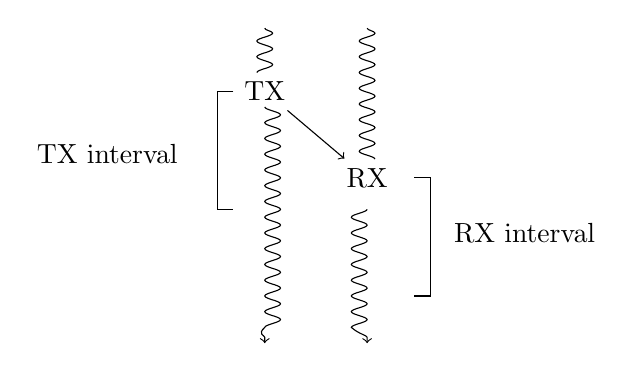
\begin{tikzpicture}
      \draw[->,decorate,decoration={snake,segment length=2mm, amplitude=1mm}]
        (0mm,0mm) -- (0,-5mm)
        (0mm,-8mm) node (TX) {TX} (0,-10mm) --
        (0mm,-40mm);
      \draw (-4mm,-8mm) -- (-6mm,-8mm) -- (-6mm,-23mm) -- (-4mm,-23mm);
      \draw (-20mm,-16mm) node {TX interval};

      \draw[->,decorate,decoration={snake,segment length=2mm, amplitude=1mm}]
        (13mm,0mm) -- (13mm,-16mm)
        (13mm,-19mm) node (RX) {RX} (13mm,-23mm) --
        (13mm,-40mm);
      \draw (19mm,-19mm) -- (21mm,-19mm) -- (21mm,-34mm) -- (19mm,-34mm);
      \draw (33mm,-26mm) node {RX interval};
      \draw[->] (TX) -- (RX);
    \end{tikzpicture}
  \end{minipage}
  \begin{minipage}{50mm}
    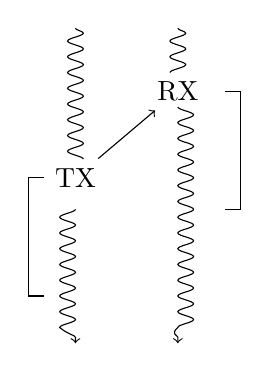
\begin{tikzpicture}
      \draw[->,decorate,decoration={snake,segment length=2mm, amplitude=1mm}]
        (0mm,0mm) -- (0,-16mm)
        (0mm,-19mm) node (TX) {TX} (0,-23mm) --
        (0mm,-40mm);
      \draw (-4mm,-19mm) -- (-6mm,-19mm) -- (-6mm,-34mm) -- (-4mm,-34mm);

      \draw[->,decorate,decoration={snake,segment length=2mm, amplitude=1mm}]
        (13mm,0mm) -- (13mm,-5mm)
        (13mm,-8mm) node (RX) {RX} (13mm,-10mm) --
        (13mm,-40mm);
      \draw (19mm,-8mm) -- (21mm,-8mm) -- (21mm,-23mm) -- (19mm,-23mm);
      \draw[->] (TX) -- (RX);
    \end{tikzpicture}
  \end{minipage}
  \begin{minipage}{80mm}
    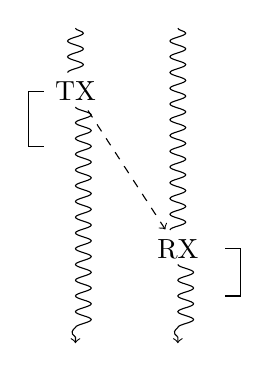
\begin{tikzpicture}
      \draw[->,decorate,decoration={snake,segment length=2mm, amplitude=1mm}]
        (0mm,0mm) -- (0,-5mm)
        (0mm,-8mm) node (TX) {TX} (0,-10mm) --
        (0mm,-40mm);
      \draw (-4mm,-8mm) -- (-6mm,-8mm) -- (-6mm,-15mm) -- (-4mm,-15mm);

      \draw[->,decorate,decoration={snake,segment length=2mm, amplitude=1mm}]
        (13mm,0mm) -- (13mm,-25mm)
        (13mm,-28mm) node (RX) {RX} (13mm,-30mm) --
        (13mm,-40mm);
      \draw (19mm,-28mm) -- (21mm,-28mm) -- (21mm,-34mm) -- (19mm,-34mm);

      \draw[->,dashed] (TX) -- (RX);
    \end{tikzpicture}
  \end{minipage}
  \caption{Overlapping TX and RX intervals allow the message to be
    sent, regardless of which operation is ordered first.}
  \label{fig:enforce:message_windows}
\end{figure}

\begin{algorithmic}[1]
  \If {The low-level interpreter has a bound interpreter}
    \If {The bound interpreter is not attempting to send a message}
      \State {Wait for it to do so}
    \EndIf
    \State {Set $s'$ to the bound interpreter's outgoing message}
  \Else
    \State {Collect all outstanding unbound send operations as the set $s$}
    \State {Extend $s$ with $\bot$}
    \State {Choose $s'$ non-deterministically from $s$}
    \If {$s' = \bot$}
      \State {Register the interpreter as a receiver of unbound messages}
      \State {Wait for the RX interval}
      \State {Unregister the interpreter as a receiver of unbound messages}
      \State {Collect all outstanding unbound send operations as the set $s$}
      \State {Select $s'$ non-deterministically from $s$}
    \EndIf
  \EndIf
  \If {$s'$ passes the side condition}
    \State {Discharge the message, unblocking the bound interpreter and moving to the Emul state}
  \Else
    \State {The plan has failed and the interpreter exits}
  \EndIf
\end{algorithmic}

The send operation is symmetric:

\begin{algorithmic}[1]
  \If {The low-level interpreter has a bound interpreter}
    \If {The bound thread is not attempting to receive a message}
      \State {Wait for it to do so}
    \EndIf
  \Else
    \State {Collect all outstanding unbound receive operations as the set $s$}
    \State {Extend $s$ with $\bot$}
    \State {Choose $s'$ non-deterministically from $s$}
    \If {$s' = \bot$}
      \State {Register the interpreter as a sender of unbound messages}
      \State {Wait for the TX interval}
      \State {Unregister the interpreter as a sender of unbound messages}
      \State {Collect all outstanding unbound receive operations as the set $s$}
      \State {Select $s'$ non-deterministically from $s$}
    \EndIf
  \EndIf
  \If {$s'$ passes the side condition}
    \State {Discharge the message, unblocking the bound interpreter and moving to the Succ state}
  \Else
    \State {The plan has failed and the interpreter exits}
  \EndIf
\end{algorithmic}

The behaviour when $s' = \bot$ is perhaps somewhat surprising: the
thread waits a little while and then selects a peer thread to
discharge the message with non-deterministically.  Meanwhile, all of
the other threads are simultaneously performing similar
non-deterministic choices.  The use of look-ahead nondeterminism means
that all of the threads will make these selections in a mutually
compatible way, so that there is no danger of A attempting to
discharge its message with B while B discharges with C.  The actual
implementation must resolve these constraints much more carefully, and
is discussed in detail later.

\todo{Defer this para until I've explained about interpreter
  duplication.}  Note that the side condition is evaluated as the
message is being discharged, while the two interpreters are merged.
It is possible to imagine an alternative implementation in which
discharging the message copies enough state from the transmitting
interpreter to the receiver to allow the condition to be evaluated
locally in the receiver after the interpreters have been unmerged.
This would reduce the size of the synchronised section and so would
appear, on the face of it, to offer greater parallelism, and hence
potentially better performance.  Unfortunately, it does not work.  To
illustrate the problem, consider again the example shown in figure
\todo{...}.  One thread modifies a shared structure while another
thread reads it, and the program will crash if the two threads happen
to be operating on the same structure at the same time.  Suppose that
the read thread runs far more often than the write one and that there
are many instances of the structure.  The timeout balancing logic will
quickly reduce the delay on the read side's first message send to zero
and increase the delay on the write side's first message receive to
compensate.  Now, when the write interpreter does run it will stop
just before \verb|l9| waiting for a matching read interpreter to
arrive.  By hypothesis, many such interpreters will arrive, as the
read thread runs more often than the write one.  In the alternative
design, the side condition can only be evaluated in the receiving
interpreter once the message operation is complete.  In this case the
receiving interpreter is the write thread, and so every read
interpreter will be forced to bind to the write thread.  Only one
interpreter can be bound to the write thread at any one time, and so
satisfying these later attempts to bind will force the write
interpreter to be duplicated many times.  Because of timeout
rebalancing, the read interpreter will proceed from \verb|l2|
immediately and quickly reach \verb|l5|, where it has to receive a
message from \verb|l9|.  At this point, there are two possible
outcomes:

\begin{itemize}
\item
  The read interpreter is delayed at \verb|l5| waiting for the message
  from \verb|l9|.  The write interpreter is still waiting in case any
  other threads reach \verb|l2| and attempt to synchronise with it,
  and so this might potentially be a rather long delay.  Since the
  read thread runs far more often than the write thread, this will
  have a very large performance impact.  Worse, it will probably be
  pointless: there are, by hypothesis, a large number of instances of
  the structure which is being examined, and so, with high
  probability, the write thread will be modifying a different one.
  When the write interpreter does finally escape from its receive
  delay and evaluate the side condition it will discover that the
  filter fails, and so the write thread will exit.  The read thread
  will then discover that its bound thread has exited and be forced to
  exit as well.  The crash enforcement plan will therefore not
  complete and the bug is highly unlikely to reproduce.
  
  Even worse, the performance hit might mean that the read thread will
  run far less frequently, further reducing the likelihood of the bug
  reproducing.  In extreme cases, the attempt at enforcing a crash
  might actually make the bug less likely to reproduce per unit time.
\item
  The thread is not delayed at \verb|l5|.  It never receives the
  message from \verb|l9| and must therefore exit without completing
  the plan, so is unlikely to reproduce the bug.  The write thread's
  high-level interpreter will then accumulate a collection of
  low-level threads which have bound to exited read threads and which
  will themselves immediately exit.
\end{itemize}

Neither outcome helps to reproduce the target bug.

By contrast, in the scheme used by SLI, the read thread is able to
evaluate the side condition at \verb|l2| and will therefore only bind
to write threads which modify the structure which it is reading.  That
means that the thread can be delayed a relatively long time at
\verb|l5| without fear of apocalyptic performance damage, and so the
bug will reproduce relatively easily.

\subsubsection{Timeout balancing}

Selecting the size of the various timeouts is important for
determining the likelihood of reproducing a bug and the overheads of
enforcing the patch.  SLI does so primarily dynamically, in response
to the program's observed behaviour.  I now consider briefly how these
timeouts should be set.

By far the most important timeouts are those which occur when unbound
interpreters synchronise, as bound-interpreter delays only happen when
the bug is already quite likely to reproduce\editorial{kind of}, so
assume for now that those are the only two delays.  There are two such
delays, one for sending the first message and one for receiving it.
Call them $D_1$ and $D_2$.  Assume that the two CFGs occur randomly
with rates $R_1$ and $R_2$.  Now the overhead introduced by the delays
is $D_1.R_1 + D_2.R_2$.  Ignoring side conditions, the bug will be
reproduced if the two CFGs occur such that the intervals on their
initial message operations overlap; in other words, if they occur with
time $D_1 + D_2$ of each other.  To put it another way, each
occurrence of CFG 2 defines a window in the execution of size $D_1 +
D_2$ such that the bug will reproduce if CFG 1 starts anywhere in that
window.  CFG 1 starts randomly with rate $R_1$, and so the probability
of any give instance of CFG 2 reproducing the bug is roughly $R_1(D_1
+ D_2)$, provided CFG 1 is sufficiently rare that we can neglect the
probability of two instances occurring in the window.  The expected
rate of bug reproduction is therefore $R_1.R_2.(D_1+D_2)$.  Some
simple algebra then allows us to show that if the desired overhead is
$k$, the reproduction rate will be

\begin{displaymath}
\alpha = k.R_2 + R_2.D_2(R_1 - R_2)
\end{displaymath}

So that if $R_1 > R_2$ the reproduction rate for a given level of
overhead is maximised by setting $D_2$ as large as possible, and
conversely if $R_2 > R_1$ the rate is maximised by setting $D_2$ as
small as possible.  In other words, if the total delay is fixed, it
should always all be apportioned to one side of the message operation.
{\Technique} therefore keeps a counter of how many times the send and
receive sides of each message operation are attempted; if the send
operation has been attempted more times than the receive one then the
send operation delay is set to zero, and otherwise the receive delay
is set to zero.

\todo{Talk about how to set the delay when we've not decided that it
  needs to be zero.}

\subsubsection{Implementing non-deterministic choice in the Succ phase}

It might be that an instruction has several possible successors in the
control flow graph in the crash execution plan, and in that case the
interpreter must choose one of these successors using look-ahead
non-determinism.  This cannot be implemented in any
physically-realisable system, as it is non-causal, and so SLI must
emulate it.  SLI uses a power-set construction to do so.  Rather than
operating a single interpreter context, the actual implementation
maintains a set of low-level interpreter contexts, which individually
follow the abstract semantics given above, and interprets them all in
lock-step parallelism.  When one of these low-level interpreters needs
to perform a non-deterministic choice between $n$ possible values, the
high-level interpreter creates $n$ successor low-level interpreter
states, one corresponding to each possible outcome of the choice, and
inserts all of them into its current-state set.  They are then
interpreted in parallel until enough information is available to
resolve the earlier choice, at which point all but one of the threads
will exit and the interpreter can revert to ``single-threaded''
execution mode.  If a thread is bound when it performs a
non-deterministic choice then its bound thread must also be
duplicated, to ensure that the new thread has something to bind to.

One subtlety here is that the original program's underlying
instruction can only be retired once, and so the high-level
interpreter must ensure that all low-level interpreters arrive at that
point in the execution cycle at the same time.  SLI actually enforces
a slightly stronger constraint, which is that every low-level
interpreter in a given high-level interpreter must be at the same
phase in the instruction execution cycle.  The semantics given above
is designed to ensure that this always possible.  The only phases for
which it is difficult are the message send and receive phases, which
are discussed in more detail in the next section.

\subsubsection{Concrete implementations of message send and receive}

The abstract semantics given above for message send and receive
operations is not realisable on any physical hardware as it relies on
non-causal nondeterministic lookahead.  Moreover, the power-set
construction used to resolve the non-deterministic Succ state is not
sufficient here as the message operation involves a sleep operation,
and hence has non-revocable externally visible side effects.  Solving
this problem requires the message operation to be ``turned inside
out'', restructuring it into a fragment which occurs before the sleep
and another fragment which occurs after it with the remaining
non-determinism confined to the two fragments.  The resulting message
receive operation looks like this:

\begin{algorithmic}[1]
  \State {$lls \gets $ the set of currently-active low-level interpreter states}
  \State {$newLls \gets $ an empty set of low-level interpreter states}
  \For {$l$ in $lls$}
    \If {$l$ does not receive any messages}
      \State {Move $l$ from $lls$ to $newLls$ without changing it}
    \ElsIf {$l$ has a bound thread}
      \If {$l$'s bound thread has exited}
        \State {$l$ exits as well; remove it from $lls$ without adding it to $newLls$}
      \ElsIf {$l$'s bound interpreter's sending-bound-message flag is set}
        \If {The bound interpreter's outgoing message passes any side condition}
          \State {Move $l$ from $lls$ to $newLls$}
          \State {Clear the bound interpreter's sending-bound-message flag}
        \Else
          \State {$l$ exits; remove it from $lls$}
        \EndIf
      \Else
        \State {Set $l$'s receiving-bound-message flag}
      \EndIf
    \Else \Comment{Unbound receive}
      \For {$s$ registered unbound senders}
        \If {$s$'s outgoing message passes the side condition}
          \State {$l' \gets $ duplicate $l$}
          \State {$s' \gets $ duplicate $s$}
          \State {Bind $l'$ and $s'$ together}
          \State {Insert $l'$ into $newLls$}
          \State {Insert $s'$ into $s$'s high-level interpreter's active low-level interpreter list}
        \EndIf
      \EndFor
      \State {Register $l$ as an unbound receiver}
      \State {Set the minimum delay to the receive operation's delay, if it is currently less than that.}
    \EndIf
  \EndFor

  \If {$lls$ is empty}
    \State \Return
  \EndIf

  \State {$end \gets now() + bound\_delay$}
  \If {There is a minimum delay}
    \State {Sleep for the minimum delay}
  \EndIf

  \While {There are bound receives in $lls$ and $now() < end$}
    \State {Wait for some bound receive to complete, or for the current time to pass $end$}
    \For {$l$ performing bound receives in $lls$}
      \If {$l$'s bound thread has exited}
        \State {Remove $l$ from $lls$}
        \State {$l$ exits}
      \ElsIf {$l$'s receiving-bound-message flag is clear}
        \State {Remove $l$ from $lls$}
        \State {Add $l$ to $newLls$}
      \Else
        \State Continue waiting
      \EndIf
    \EndFor
  \EndWhile

  \For {$l$ in $lls$}
    \If {$l$ is registered as an unbound receiver}
      \State {Unregister $l$ as an unbound receiver}
    \EndIf
    \If {$l$'s receiving-bound-message flag is set}
      \State {Exit $l$} \Comment{Receiving bound message failed}
    \ElsIf {$l$ is unbound}
      \State {$l$ must have been attempting an unbound receive which failed, so it exits}
    \Else
      \State {Add $l$ to $newLls$}\Comment {Receive succeeded}
    \EndIf
  \EndFor
\end{algorithmic}

For clarity, I have omitted the synchronisation on the various
interpreter-internal structures.  The send algorithm is symmetrical,
simply replacing the word ``receive'' with the word ``send'' and vice
versa.  There are a couple of features to note in this algorithm:

\begin{itemize}
\item
  If there are any unbound message operations then it waits for the
  whole of that message's delay, even if some other interpreter which
  might match the operation arrives.  This reflects the semantics
  already discussed in which any message operation will synchronise
  will all other matching operations in its window.  On the other
  hand, it can lead to poor performance, and the slight loss of
  correctness from ending the wait early is very rarely important.
  \todo{Say more.}
\item
  When interpreters are bound together both interpreters are
  duplicated.  This means that the original interpreter is left in the
  unbound send state, and can therefore synchronise with any
  additional interpreters which might arrive.
\item
  Bound messages use a different delay strategy to unbound ones.  This
  is because bound operations fail in different ways.  By
  construction, a bound interpreter will eventually either exit or
  perform all planned message operations and so it might appear that
  bound operations should never hit there timeout, and that is indeed
  the common case.  It is, however, possible, albeit very rare, for
  {\technique} enforcers to introduce a deadlock if they interact
  badly with the program's existing synchronisation structure.  These
  timeouts avoid that issue.  \todo{Actually, now I think about it, I
    don't think that deadlock is actually possible.}
\end{itemize}

One further optimisation, not shown here but implemented in
{\implementation}, avoids redundantly duplicating low-level
interpreter contexts in the common case that a message operation is
discharged precisely once.

\todo{This is probably not the best way of presenting those
  algorithms.}

\subsubsection{Starting new low-level interpreters}

The high-level interpreter is responsible for starting new low-level
interpreters as the program under test moves through CFG nodes which
are marked as entry point nodes.  This might be because the program
has just reached one of the interpreter entry point instructions,
already discussed in the discussion of building patch strategies.  It
might also be because the program has reached an entry point while
running under the interpreter, in which case the high-level
interpreter must start another low-level interpreter to handle the new
CFG.  This can happen if the one of the CFG fragments is
cyclic\editorial{Or as cyclic as the unrolled CFG fragments ever
  get...} and re-enters itself, or if two of the CFG fragments
overlap.  {\Implementation} handles either case correctly.

After starting a new low-level interpreter the high-level interpreter
must run any entry point side conditions, as already discussed, and
stash the value of any $LD$ or register expressions which are needed
later on.

\subsubsection{The await-bound-thread-exit state}

When a thread completes its plan, it is sometimes useful for it to
wait for its bound thread to exit before proceeding.  This is because
the crash summary from which the plan is generated does not have
complete information on the structure of the program and can miss
relevant stores which happen after the write-side {\StateMachine}
completes.  If the last edge in a happens-before graph is from memory
access A to memory access B, that usually means that A is a store and
B is a load and B must load the value stored by A.  That means that,
not only must B happen after A, but B must happen before any other
writes to the memory location modified by A.  If there were other
stores to that location in the crash summary then the happens-before
graph would include additional edges to ensure that that happens, but
if there are stores outside of the analysis window then it will not.
For instance, suppose that the write thread looks like this:

\begin{verbatim}
while (1) {
l1:  *x = 5;
l2:  *x = 7;
     <something_complicated>
}
\end{verbatim}

And the read thread looks like this:

\begin{verbatim}
l3: a = *x;
l4: b = *x;
    crash if a != b;
\end{verbatim}

This program is clearly buggy.  One way of reproducing this bug would
be to interleave instructions as \verb|l1|, \verb|l3|, \verb|l2|,
\verb|l4|, and SLI will discover this interleaving as the
happens-before graph show in figure~\ref{fig:enforce:await_exit_hb}.
The algorithm described so far will be sufficient to enforce this
graph (assuming that the two fragments of code shown can actually
execute in parallel) but may still struggle to reproduce the bug.
This is because the generated happens-before graph is incomplete: it
misses the edge from \verb|l4| to \verb|l1| in the next iteration of
the loop.  If the loop completes and reaches the store at \verb|l1|
before the load \verb|l4| completes then the bug will not reproduce
even though the happens-before graph was successfully enforced.  Any
scheme with an analysis horizon based on a simple instruction count
will suffer from a similar problem, but this is particularly serious
for SLI, because the delays inserted are in almost precisely the right
place to maximise the chance of this kind of bug-hiding race.  In the
example, the crash enforcement plan will include a message send edge
\verb|l2| to \verb|l4| so that \verb|l4| will block waiting for
\verb|l2| to complete.  When \verb|l2| completes, it will unblock
\verb|l4| and then immediately return, and the two threads will race
to see whether \verb|l4| will complete before \verb|l1| has a chance
to run again.  Usually, the latency of unblock a thread is large
relative to even quite long sequence of ordinary instructions, and so
with very high probability \verb|l1| will execute before \verb|l4| and
hide the bug.  This bug will therefore never reproduce under SLI's
crash enforcer, even when the happens-before graph is enforced
perfectly.  The fix is simple: have the store thread delay slightly
after completing its final message send operation until the read
thread also completes its crash enforcement plan.  This ensures that
activity beyond the analysis horizon cannot prevent bug reproduction,
and, because it only happens when the plan is mostly complete, and
hence happens very rarely, it has very low performance overhead.

\begin{figure}
\begin{tikzpicture}
\node[CfgInstr] (l1) {l1};
\node[CfgInstr, below = of l1] (l2) {l2};
\node[CfgInstr, right = of l1] (l3) {l3};
\node[CfgInstr, below = of l3] (l4) {l4};
\draw[->] (l1) -- (l2);
\draw[->] (l3) -- (l4);
\draw[->,happensBeforeEdge] (l1) -- (l3);
\draw[->,happensBeforeEdge] (l3) -- (l2);
\draw[->,happensBeforeEdge] (l2) -- (l4);
\end{tikzpicture}
\caption{Happens before graph for the await-bound-exit example.}
\label{fig:enforce:await_exit_hb}
\end{figure}

\subsection{Combining multiple enforcers}
\label{sect:enforce:combine_enforcers}

The initial static analysis and symbolic execution phase can generate
a large number of false positives, and it would be extremely tedious
to have to test each one independently.  {\Implementation} therefore
includes a mechanism for enforcing multiple bugs at once.


\subsection{Compiling the plan}
\label{sect:enforce:compiling}

\todo{Implementation of this is currently massively broken; need to
  decide whether I'm going to fix it or just use a slightly older
  version, or just drop it completely.  Also, some of the
  simplifications to the semantics described here aren't really
  necessary or well thought-through.}

In addition to a plan interpreter, SLI also includes a plan compiler, which combines the plan with the program's original machine code to produce a modified version of the program which performs the necessary enforcement actions without needing an interpreter.
The intent here is to reduce the overhead of the interpreter in the case where SLI is investigating many bugs most of which do not exist.
Making this practical requires several simplifications to the semantics:

\begin{itemize}
\item
  The number of physical program threads operating in the plan is limited.
  In particular, it is assumed that only one program thread will be executing the read side of the plan at any time, and likewise only one thread will be executing the write side.
\item
  The message semantics are simplified: messages are sent asynchronously, with a delay only on the read side, and must be ``cancelled'' when the relevant thread exits.
  This has two important implications: first, that a message send can never fail and, second, the something must keep track of what messages a given thread currently has outstanding.
  Combined with the first simplification, it also means that at most one instance of any given message can be outstanding at any one time, and so it is easy to place the relevant information in a global structure without needing any dynamic memory allocation.
\item
  High-level interpreter contexts only ever access the state of their own low-level interpreters.
  This has two important implications:

  \begin{itemize}
  \item
    Remote low-level interpreters are never duplicated during message operations.
    If the normal semantics would require an interpreter to be duplicated then the local message operation fails.
  \item
    The receive message filter can only be executed by the receiving thread after receiving a message.
  \end{itemize}
\item
  When a low-level interpreter is duplicated due to a non-deterministic choice in the Succ phase the low-level state's stash table is not duplicated.
  Instead, all low-level interpreters in a given high-level interpreter share a single stash table.
\end{itemize}

The result is a system with lower run-time overheads, but also a lower probability of reproducing interesting bugs.
It has a much larger I-cache footprint but a smaller D-cache one\editorial{Not sure where I'm going with that, although it is true and kind of interesting}.

I now briefly outline the implementation of this compiler.
The core idea is to compile the CFG in the enforcement plan into a state machine.
This state machine consists of a large number of smaller intra-instruction state machines, as illustrated in figure~\todo{...}, each of which models a single instruction in the original program.
The label on each state is itself a set of low-level labels which consist of a four-tuple of the plan thread which is executing, a reference to the plan CFG node, a set of messages which have been sent by the thread, and the phase of the intra-instruction state machine.
Each state is compiled to a small fragment of machine code (which might be empty, if this instruction does not have an relevant annotation in the plan) plus a set of relocations specifying the fragment's relationships to the other states.
Once every state has been compiled these relocations can be discharged and the fragments concatenated together to form the final patch.

I now discuss the details of each phase of the intra-instruction machine:

\begin{itemize}
\item[RecvMsg]
  Examine the set of CFG nodes which are active in the current state and determine whether the plan requires any of them to receive messages.
  If so, emit code to examine the global outstanding-message structures to see whether of the desired messages are currently outstanding.
  If there are, receive precisely that message.
  Any other message receive operations are considered to have failed and the relevant CFG nodes removed from the current state label.
  If no message sends are currently outstanding then the physical thread is delayed until either one is available or some timeout is reached.
  If a message becomes available then it is received, and otherwise all receives fail and all receiving CFG nodes are removed from the label.
  Note that this does not necessarily mean that the state label will become empty\footnote{Although that is the common case.} as there may be some CFG nodes which do not need to receive messages.

  Once a message is received its content is simply copied from the global message area into the local thread's stash area.
\item[OrigInstr]
  Store any generated values into simulation slots and issue the original instruction.
  There are three main cases to consider here:

  \begin{itemize}
  \item
    Simple memory loads.
    If the instruction is of the form \verb|LOAD *location -> register|, and the value loaded is to be saved, then it is sufficient to just copy \verb|register| into the simulation slot after the original instruction has completed.
  \item
    Compound memory loads.
    Instructions which load from memory but are not themselves simple loads are more difficult to handle.
    For concreteness, suppose that the instruction is \verb|CMP 76,*loc1|, and the annotation requires us to save the value loaded.
    The instruction loads from \verb|*loc1| but does not leave the result in any locations which we can easily access.
    It would be possible to solve this problem by adding another load of \verb|*loc1|, but that would run the risk of a store in a remote thread modifying \verb|*loc1| between the two loads, leading to very confusing results.
    SLI instead solves this problem by rewriting the instruction to this:

\begin{verbatim}
LOAD *loc1 -> reg1
STORE reg1 -> simslot
CMP 76, reg1
\end{verbatim}

    This exposes the loaded value to the instrumentation framework, allowing it to be stored to the simulation slot as desired.

    Instructions which modify memory in-place, such as \verb|ADD 1 + *loc1 -> *loc1|, pose a similar problem and can be solved in the same way, provided that they do not have a \verb|LOCK| prefix.
    \verb|LOCK|ed instructions are more complex, as separating the load and store phases into separate instructions would violate the semantics of the program and might introduce new bugs.
    SLI solves this problem using a \verb|CMPXCHG| loop.
    For instance, the instruction \verb|LOCK ADD 1 + *loc1 -> *loc1| would be converted to this machine code fragment:

\begin{verbatim}
1: LOAD *loc1 -> reg1
ADD 1 + reg1 -> reg2
LOCK CMPXCHG *loc1, reg1 -> reg2
if_cmpxchg_failed goto l1
STORE reg1 -> simslot
\end{verbatim}

    The \verb|CMPXCHG| instruction here is supposed to be an invented syntax for the x86 machine code instruction which atomically compares \verb|*loc1| to \verb|reg1| and, if they are equal, sets \verb|*loc1| to \verb|reg2|.
    This allows SLI to expose the value of the implicit load while preserving the \verb|LOCK| semantics of the original instruction.
  \item
    Branch instructions are deferred to the FindSucc state.
  \end{itemize}
  
\item[SendMsg]
  Send any outgoing messages.
  This amounts to simply copying the message payload into the global message area, setting a global flag to indicate that the message is currently outstanding, and adding the message ID to the state label's set of sent messages.
  This always succeeds and advances to the FindSucc state.

\item[ExitThread]
  When a low-level thread exits it is necessary to cancel any messages which it has sent.
  The compiler takes the union of all of the sent-messages sets in its low-level, removes the thread which is to exit, and then takes the union again.
  Any messages present in the first set but not the second need to be cancelled by setting the relevant global message-outstanding flag to zero.
  The compiler will then either exit the patch, if the last low-level thread has exited, or resume the intra-instruction state machine at an appropriate place.
\end{itemize}


\begin{tikzpicture}
\node[flowChartState] (RecvMsg) {RecvMsg};
\node[flowChartState,above left = of RecvMsg] (StartThread) {StartThread};
\node[flowChartState,above right = of RecvMsg] (CheckForThreadStart) {CheckForThreadStart};
\node[flowChartState, below = of RecvMsg] (OrigInstr) {OrigInstr};
\node[flowChartState, below = of OrigInstr] (VerfCond) {VerfCond};
\node[flowChartState, below = of VerfCond] (SendMsg) {SendMsg};
\node[flowChartState, below = of SendMsg] (FindSucc) {FindSucc};
\node[flowChartState, right = of VerfCond] (CondFail) {CondFail};
\node[flowChartState, right = of CondFail] (Exit) {Exit};
\node[flowChartState, left = of RecvMsg] (RecvdMsg) {RecvdMsg};
\draw[->] (CheckForThreadStart) -- (RecvMsg) -- (OrigInstr) -- (VerfCond) -- (SendMsg) -- (FindSucc);
\draw[->] (StartThread) to [bend right=10] (CheckForThreadStart);
\draw[->] (CheckForThreadStart) to [bend right=10] (StartThread);
\draw[->,dashed] (FindSucc.east) to [bend right=75] (CheckForThreadStart.east);
\draw[->] (RecvMsg) -- (RecvdMsg) -- (OrigInstr);
\draw[->] (RecvMsg) -- (Exit);
\draw[->] (VerfCond) -- (CondFail) -- (Exit);
\draw[->] (FindSucc) -- (Exit);
\end{tikzpicture}

  

\subsubsection{Run-time considerations}

Evaluating side conditions is not always completely trivial, even once
all of the inputs are available.  In particular, $LD(addr)$
expressions require a moderate amount of care.  These are defined to
return the state of memory when the {\StateMachine}, and hence the
CFG, starts.  The problem is that the address might turn out to be a
bad pointer, and it is important for the enforcer not to cause the
program to crash in that case.  {\Implementation} solves this problem
by simply catching page faults generated while evaluating side
conditions.  If any such faults occur then the relevant low-level
interpreter state is considered to have failed.  This is not always
ideal from the point of view of reproducing the bug, but avoids
spuriously crashing the program under test.

\todo{Why do we sometimes end up dereferencing pointers which the
  program never does? Answer: because the placement stuff sometimes
  ends up pulling validation over program control flow, which makes it
  easier to implement and easier to fast-out of the enforcer, but
  risks introducing these bad dereferences.}

\subsection{Comparison to schedule memoisation}
\subsection{Comparison to STM block inference stuff}

\section{Fixing bugs}

\subsection{Using global locks}
\label{sect:fix_global_lock}

In addition to finding bugs, SLI can also be used to fix them in a
largely automated fashion.  The basic approach here is to binary patch
the program to introduce a new global lock covering the program's
relevant instructions, preventing them from executing in parallel and
hence preventing the bug from occurring (assuming that the relevant
instructions have been correctly identified).  The relevant
instructions are duplicated into a binary patch, unrolling loops and
tracing across function boundaries in a way which reflects the
function inlining and loop unrolling performed during the initial CFG
generation phase, and the duplicates modified to acquire and release
the lock at appropriate points.  The original program is then patched
to branch to the duplicates when necessary.

The first step in producing such a fix is correctly identifying the
instructions which must be included in the critical sections.  These
will be roughly a subset of the instructions involved in the
control-flow graphs associated with \StateMachines; a subset because
some instructions in the CFG do not need to be protected, and roughly
because some instructions not in the CFG will also be included in the
critical section.

As an example of the former, consider a program like this:

\begin{verbatim}
read_side() {
    ptr = complicated_local_calculation();
    dptr = *ptr;
    if (dptr != NULL) {
       dptr = *ptr;
       *dptr = 5;
    }
}
write_side() {
    ptr = complicated_local_calculation();
    *ptr = NULL;
}
\end{verbatim}

Here, the read thread computes some pointer using entirely local
operations, loads from it once and then, if the result is
non-\verb|NULL|, loads from it again and uses the resulting pointer.
Meanwhile, the store thread sets a potentially coincident memory
location to \verb|NULL|.  The read thread clearly has a potential
time-of-check, time-of-use race bug.  The \StateMachines generated by
SLI will include the buggy code itself but might also include part or
all of \verb|complicated_local_calculation()| and a side-condition
which requires the two pointers to match up.  This extra information
is useful when analysing the bug (\needCite) or when attempting to
reproduce it (\needCite) but cannot be used by this kind of
instruction-level fix\footnote{But see future work section~\needCite
  for a possible alternative scheme which would make use of it.}, so
including it in the fix is unhelpful and would tend to lead to
unnecessarily large critical sections.  The fix generating process
must therefore select a useful subset of the instructions in the
control-flow graph.

The approach taken here is simple:

\begin{itemize}
\item
  Extract all of the happens-before edges from the bug summary's
  verification condition.  These entirely capture the
  instruction-interleaving parts of the bug to be fixed, and, since
  instruction-interleaving is the only thing which can be influenced
  by this type of patch, the resulting set of edges contains all of
  the useful information in the condition.
\item
  Identify all of the CFG nodes which are mentioned in one of those
  happens-before edges.
\item
  Trim the CFG such that every path starts and ends in one of those
  mentioned nodes.  All such paths will be included in a critical
  section, and so no such paths will be permitted to execute in
  parallel.
\end{itemize}

In this way the CFG is restricted to just those instructions which are
involved in the interleaving which is to be prevented.

Note that this is not guaranteed to produce an optimal selection of
critical sections, in the sense that sections can sometimes be larger
than is strictly necessary.  Consider, for example, a program with the
same read side as the previous example but a write side in which the
pointer is assigned to twice:

\begin{verbatim}
write_side() {
    ptr = complicated_local_calculation();
    *ptr = NULL;
    *ptr = NULL;
}
\end{verbatim}
    
There are now two obvious ways of protecting this program:

\begin{itemize}
\item
  Place both loads in the read side in a single critical section and
  both stores in the write side in another one.
\item
  Place both loads in the read side in a single critical section, but
  give each store in the write side its own critical section.  In
  other words, drop and re-acquire the lock in between the two stores.
\end{itemize}

Both approaches correctly eliminate the bug, but they will have
different performance characteristics.  In particular, dropping and
re-acquiring the lock reduces the size of the critical section, which
might improve concurrency and reduce starvation, but imposes higher
overheads due to the greater number of lock operations.  In principle
the happens-before graph implicit in the verification condition
contains enough information to determine whether dropping the lock is
safe, but, in this mode, SLI does not make use of this information,
and always uses the former strategy\footnote{But
  see~\ref{sect:fix_from_drs} for a mode in which it can use the other
  approach.}.

Once the relevant fragment of CFG has been identified, entry point
stubs must be generated and the program patched to branch to them at
appropriate points.  The difficulties involved in placing branch
instructions has already been discussed, in the context of enforcing
crashes, and will not be discussed again here.  As in the crash
enforcement case, simply gaining control on the right instructions is
insufficient here, as the calling context of the instruction must also
be checked.  The approach here is again similar to that used for
enforcers, except that the stack offsets are compiled into a fragment
of machine code which performs the necessary checks rather than being
turned into a table which can be checked by an interpreter.

One subtlety here is that the patches do not have the ability to
recover from artificially introduced bad pointer dereferences, and so
must be careful to never touch any potentially bad memory which is not
also touched by the original program.  This potentially includes
accessing stack locations, if the context to be validated is for a
very deep stack and the current program location has a very shallow
stack.  {\Technique} avoids this issue by always validating stacks
from the bottom up, so that functions nearer the current location in
the stack are checked first.  This means that when the return address
of a function $f$ is checked, the checker has already made sure that
$f$ is actually on the stack in the expected place, and so it can be
certain that $f$'s return address is also available in the expected
place\footnote{One obvious exception would be functions whose stack
  frame size can change, but these already defeat the stack layout
  discovery algorithm and so no patch can be generated for them
  anyway.}.

A further minor consideration is performance.  If we have to validate
several similar contexts then we generally want to avoid testing the
same memory locations more times than is necessary.  The validation
machine code is therefore structured as a tree of case splits on the
set of possible contexts with leaves corresponding to specific
contexts.

A further complication is that, even once the patch has been entered,
it is not always completely clear which CFG node the program is
actually executing.  There are a number of reasons for this:

\begin{itemize}
\item
  There might be some entry context which is a subset of another entry
  context.  For instance, the fix generator might be asked to protect
  one CFG which starts in context $g$, $f$, where $f$ is the top of
  the stack, and another which starts in context $h$, $g$, $f$.  If
  the context validation finds that the initial context is $h$, $g$,
  $f$ then both CFGs should start.
\item
  One of the CFG fragments to be protected might contain the starting
  point of another CFG fragment, and both CFGs should be fully
  protected.  This means that the lock cannot be dropped until both
  are certain to have ended.  At the same time, it is important that a
  single thread does not acquire the same lock twice, to avoid
  deadlock.
\item
  The CFG unrolling rules mean that the successor of a CFG is not
  always unambiguous anyway, and the generated patch must correctly
  handle that.
\end{itemize}

Yet a further complication is that the patch must sometimes include
some instructions which execute without holding the lock if, for
instance, the patch strategy had to include additional instructions to
avoid the branch-to-corrupt-instruction problem.

The result is that the code in the duplicated patch fragment is not
quite an exact match for that in the original program, even ignoring
the additional lock acquire and release operations.  The approach used
is similar to that used in building cross-product {\StateMachines}, as
discussed in section~\ref{sect:using:build_cross_product}.  Here, the
configurations used are drawn from the set:

\begin{displaymath}
  checkForEntry \times locked \times (rip \dot{\cup} (2^{\textrm{CFG node}} \times restoreRedzone \times finishCallSequence))
\end{displaymath}

Where $\times$ indicates cross-product, $\dot{\cup}$ indicates disjoint
union, and $2^{\textrm{CFG node}}$ indicates the power set of CFG
nodes.  It is worth explaining this in slightly more detail before
explaining the actual algorithm:

\begin{itemize}
\item $checkForEntry$ is a boolean flag indicating whether the
  labelled fragment of machine code must check for any additional
  CFGs entering the critical section.
\item $locked$ is a boolean flag saying whether the lock is
  held when the labelled machine code is entered.
\item $rip$ is the raw instruction pointer of an instruction in the
  program.  This field is present if the labelled machine code is
  implementing an instruction which is not supposed to be protected
  but was included by the patch strategy to avoid branches to corrupt
  instructions.  The labels are referred to later as ``simple''
  labels; other labels are referred to as ``compound''.
\item The set of CFG nodes indicates where abouts in the fragments
  to be protected the program is currently executing.
\item $redzone$ is a boolean flag indicating whether the AMD64
  red zone is currently present on the stack.  The red zone must be
  present whenever running any stack-accessing instructions from the
  original program but must be cleared at various points in the
  protection framework.
\item $finishCallSequence$ is either a 64 bit value which contains the
  return address of an indirect function which the patched program
  just executed.  Handling of indirect function calls is difficult
  here and is discussed in more detail later on.
\end{itemize}

The stack validation code generates an a branch to an initial label
from every leaf of its validation tree.  This initial label will be
a compound label:

\begin{itemize}
\item $checkForEntry$, $locked$, $finishCallSequence$, and $redzone$
  are all clear.
\item The set of CFG nodes is precisely the set which match the
  current call context.
\end{itemize}

I now give details of the machine code and successor labels generated
for the various relevant combinations of label and underlying
instruction.

\begin{itemize}
\item $finishCallSequence$ is the first flag checked; handling of this
  is deferred until the call sequence logic has been explained.
\item
  If the $checkForEntry$ flag is set then we generate a call context
  validation tree which checks whether any additional CFGs need to be
  started and, if so, branches to an appropriately-extended label.  In
  any case, the new label will have the $checkForEntry$ flag clear.
\item
  If the $locked$ flag is set in a simple label then code is emitted
  to drop the lock.  Likewise, if the flag is clear in a compound
  label then code is emitted to acquire it.  Acquiring or releasing
  the lock is only possible when the red zone is clear.  As a minor
  optimisation, clearing the red zone is skipped if the $redzone$ flag
  is set.  The successor label will have an appropriately-updated
  value for the $locked$ flag and the $redzone$ flag set.
\item
  If the current label is compound, but the set of CFG nodes is empty,
  the critical section has finished and the result is a branch to a
  simple label with an appropriate $rip$.
\item
  If the current label is simple, and the $rip$ is not in the $Cont$
  set of the patch strategy, the result is a simple branch back to the
  matching instruction in the original program.
\item
  If none of those tests fire then the original instruction is
  decoded.
\end{itemize}
  
\todo{There is almost certainly a better way of describing this.}
\subsection{Other ways of fixing the bugs}
\todo{I've come up with an algorithm for doing this using a message
  passing network, like we do for crash enforcement but with the
  delays in slightly different places, but I really don't have time to
  implement it.  It is kind of cool, though; I'd like to include it
  somewhere, even if it's just a future work-type thing.}

\todo{Might also be worth saying a few words about possibly fixing the
  bugs by using STM-like techniques?  I've not implemented any of
  them, either, but they are kind of interesting.  Probably worth a
  paragraph or two.}

\section{Fixing bugs from DRS logs}
\label{sect:fix_from_drs}
The simplest way to fix a bug is to start from a DRS log.
Given a log, identifying the thread and which is most responsible for a crash is generally straightforward.
If the crash is caused by dereferencing a bad pointer then the responsible thread is the one which dereferenced the pointer; if the crash is an assertion failure then the responsible thread is the one which called \verb|abort()| (or equivalent).
The log then makes it trivial to determine what instructions the responsible thread executed before it crashed, and a suffix of these can be compiled into a \StateMachine capturing the most relevant parts of the responsible thread's behaviour.

The log also makes it trivial to determine precisely which stores the read-side thread raced with, and so building a write-side \StateMachine is redundant.
Instead, the read-side \StateMachine is ``slid across'' the log, evaluating it at every step (subject to some typing constraints which ensure that the result is reasonable), and the resulting pattern of safe and unsafe regions converted directly into critical sections, without ever needing to generate an explicit write-side \StateMachines.

\subsection{Building the read-side \StateMachine}
\todo{This is gratuitously different from the non-DRS mode in an enormous number of places.  I should fix that.}

Working from a DRS log provides a lot of information which is not available in SLI's normal mode of operation.
This makes some parts of the algorithm redundant.
In particular, there is no need to generate large numbers of CFGs of fragments of the program which might be relevant, as we know precisely which instructions were executed leading up to the crash.
Instead, in this mode, SLI generates the \StateMachine directly from the log.
It starts with a small stub machine representing just the instruction which crashed and then expands it backwards, incorporating a single instruction from the log at a time.
For instance, suppose that the fragment of program to be investigated looked like this:

\begin{verbatim}
l1: mov $5, %rax
l2: mov (global1), %rbx
l3: mov (%rax + %rbx), %rcx
\end{verbatim}

and the program crashed due to dereferencing a bad pointer at \verb|l3|.
The initial stub \StateMachine will then be just:

\begin{verbatim}
if (BadPtr(rax + rbx)) crash(); else survive();
\end{verbatim}

Incorporating \verb|l2| will transform that to

\begin{verbatim}
LOAD (global1) -> rbx
if (BadPtr(rax + rbx)) crash(); else survive();
\end{verbatim}

Incorporating \verb|l1| will then produce the \StateMachine

\begin{verbatim}
COPY 5 -> rax
LOAD (global1) -> rbx
if (BadPtr(rax + rbx)) crash(); else survive();
\end{verbatim}

Which can be simplified in the usual way to produce

\begin{verbatim}
LOAD (global1) -> rbx
if (BadPtr(rbx)) crash(); else survive();
\end{verbatim}

And this can then be used in the rest of the analysis.

The major subtlety here lies in the handling of control flow, and the parts of the program which are not executed.
One possible approach would be to simply say that any changes to the control flow cause the bug to be avoided, but this is over-optimistic.
Consider, for instance, a program like this one:

\begin{verbatim}
ptr = global;
if (some_condition)
    idx = 1;
else
    idx = 2;
local = ptr[idx];
\end{verbatim}

This program loads a pointer to an array from a global variable and then loads some index in the array, with the index chosen depending on some condition.
Suppose that the race then causes the pointer in \verb|global1| to sometimes be bad, and that the reproduction of the bug was obtained while \verb|some_condition| holds.
The bug itself does not depend on \verb|some_condition|, but if one were to assume that any changes to control flow avoid the bug then SLI would not be able to show this.
This problem can only be avoided by exploring untaken branches, and SLI does so, for some (configurable) number of instructions.
If the control flow rejoins that which is represented in the DRS log then an appropriate branch is included from one part of the \StateMachine to another, and if it does not rejoin then a branch to the \verb|NoCrash| state is used instead.

One complication here is that a given static instruction might be represented multiple times in the DRS instruction trace, and hence multiple times in the \StateMachine, if the instruction is part of some loop.
This makes it ambiguous where the branch should branch to.
SLI solves this problem by taking the earliest instance of the instruction, and hence branching to the place in the \StateMachine nearest the root.
This helps to keep the loop structure of the program intact, subject to the unrolling implicit in the DRS log.

The example shown above might then turn into a \StateMachine something like this:

\begin{verbatim}
LOAD global1 -> ptr
if (some_condition) {
   COPY 1 -> idx1
} else {
   COPY 2 -> idx2
}
if (BadPtr(ptr + idx)) {
   crash();
} else {
   survive();
}
\end{verbatim}

The standard simplified will then transform that to this:

\begin{verbatim}
LOAD global1 -> ptr
if (BadPtr(ptr + (some_condition ? 1 : 2))) {
   crash();
} else {
   survive();
}
\end{verbatim}

SLI uses a rule that \verb|BadPtr(x + k)| is equivalent to \verb|BadPtr(x)| whenever \verb|k| is a small constant, and so correctly determines that the bug is independent of \verb|some_condition| in this case.

\todo{Discuss using more powerful bug definitions here e.g. Valgrind, invariant discovery, etc, by applying them to the log and then converting to stub machines, so that you can apply this to races which lead to bugs other than immediate bad pointer dereferences.}

\subsection{Requirements on the DRS}

\subsection{Finding remote critical regions}

The fixes generated by SLI rely on making the read-side \StateMachine operate as-if atomically and then ensuring that it does not execute in any states where doing so would lead to a crash.
In the normal mode of operation, the regions which would lead to a crash are determined by modelling the rest of the program as a set if write-side \StateMachines and then using symbolic execution, but it is possible to be more accurate\editorial{or possibly precise?} if a full DRS log is available.
Instead of the set of \StateMachines, the log itself can be used as a model for the rest of the program.
The idea here is that the log contains a sequence of possible states of the program, and contains all of the ones which are relevant to this particular way of reproducing the bug of interest.
SLI therefore slides the read-side \StateMachine over this log, evaluating it at every instruction, and hence classifies the log into ``safe'' and ``unsafe'' regions, and the transitions between these two types of region give the boundaries of the write-side critical regions.

As a minor optimisation, SLI only re-evaluates the \StateMachine if there has been a store to some memory location which is loaded by the \StateMachine.
This cannot affect the results in any way, but means that the \StateMachine does not have to be evaluated as often.

One important complication here is the presence of dynamically-allocated data structures.
SLI relies on being able to identify points in the program where these are allocated and released.
The loads in the read \StateMachine will correspond to specific load operations in the DRS log and SLI is then able to check which dynamic instance of structures those accesses access and will only evaluate the \StateMachine while all of the relevant structures remain live.

Once the log has been classified, the classification must be converted into realisable critical sections.
In other words, SLI must identify points in the program at which it must insert lock acquire operations and points where it must insert lock release operations.
Ideally, each unsafe region in the log would correspond to a single critical section, with a single acquire operation and a single release one.
This can fail in several ways:

\begin{itemize}
\item
  The start and end of the unsafe region might be in different threads, if, for instance, one thread violates an invariant and another thread then restores it.
  It is difficult to model a cross-thread operation as a critical section.
  SLI cannot prevent this kind of bug, and the unsafe region is simply ignored.
\item
  There might be non-trivial control flow between the start and end of an unsafe region within a single thread.
  In that case additional acquire and release operations must be inserted to ensure that locks are not leaked, double-acquired, or double-released.
\item
  The program might have additional synchronisation mechanisms which, when combined with the SLI-inferred synchronisation, lead to a deadlock.
\end{itemize}

These are discussed in more detail in \S~\ref{sect:fix_global_lock}.

\todo{This is in dire need of rewriting.}

Note that the definition of a dynamic structure is somewhat subtle here.
Most obviously, \verb|malloc| and \verb|free| represent boundaries in the lifespan of such structures (with \verb|malloc| being the start and \verb|free| being the end), but ``re-typing'' operations can also impose such boundaries.
The intent of the sliding procedure is to capture other operations which the program might perform on the data structures involved in the synchronisation bug, in the same way that write-side \StateMachines do in the non-DRS case.
In effect, the program's behaviour is constrained using a heuristic memory safety property, and this memory safety property must correspond reasonably closely to the program's actual structure.

The underlying hypothesis here is that the program has some kind of internal type system which constrains which operations will be performed on a given memory location.
This means that two pieces of code can only race if they have types which are in some sense compatible, so that they might access overlapping memory locations.
The combination of the read-side \StateMachine and the set of dynamic instances accessed by it defines, in a slightly ill-defined way, a set of types which the read side of the critical section might access.
SLI must then find some other operations on the same types to synchronise against, and this is the aim of the sliding procedure.
In order for this to work, the read \StateMachine must only be slid to places where the current types match up with the types for which it was derived.
SLI must therefore be able to identify points where the types of memory locations change.
This includes things like \verb|malloc| and \verb|free|, but is also likely to include things like program-specific memory allocators or object pools.
The precise set will depend on the program's type system, and so can only be sensibly modelled with assistance from the programmer.





